% ME310 Report Template -- Started 28 July 2006  Mark Cutkosky
% Updated: 7Aug08 -LMS; 25Nov10 Mark Cutkosky
% Updated with some new sections 4Dec2012 Mark Cutkosky
% Minor changes for 2013-14 13Nov2013 -- Mark C.
%%%%%%%%%%%%%%%%%%%%%%%%%%%%%%%%%%%

% Rename this file to whatever you like (e.g. OurFallDoc.tex) and modify the title, authors
% etc. below. If you rename the section files (e.g. Ch2context.tex) you'll need to change
% the \include{ } calls in this document as well.

%%%%%%%%%BEGIN DOCUMENT STYLE SETTINGS%%%%%%%%%%%
% Don't modify this stuff unless you know what you're doing...
% We are using the "memoir" class, a widely used set of macros book-like documents.
% If you get errors that you are missing the "memoir" package you can download and 
% install it:   http://www.ctan.org/tex-archive/macros/latex/contrib/memoir/

% memoir document class for standard USA letter paper, printed one side
\documentclass[11pt,letterpaper,oneside]{memoir}
\chapterstyle{section}
%\pagestyle{companion}    % If you want fancier page headers 
\usepackage{graphicx}        % standard LaTeX graphics 
\usepackage{color}               % support for colored fonts
\usepackage{url}  \urlstyle{same}     % deal with url strings in bibliography

\usepackage[final]{pdfpages}

%Optional fonts if you don't like the default in Latex
%\usepackage[T1]{fontenc}
%\usepackage{mathptmx}  %This will give you Times Roman, like default in MS Word.
%\usepackage{charter}       %This will give you a slightly bolder Charter font 

%More special packages to help deal with long requirements tables 
%that might span multiple pages.
\usepackage{multirow} %deal with merged cells in tables
\usepackage{supertabular}
\usepackage{longtable}
\usepackage{morefloats}
\usepackage{listings}
\usepackage{color}
\usepackage[ampersand]{easylist}

\usepackage[pdftex,           %hyperlink cross references, etc.
    pdfsubject={ME310 Documentation},
    colorlinks={true},
    linkcolor={black},
    citecolor={blue},
    bookmarksopenlevel=1,
]{hyperref}

%The file "me310.sty" should be in the same directory as this file.
% It contains formatting for page setup, titlepage, glossary, references, etc.
\usepackage{me310}
%%%%%%%END DOCUMENT STYLE SETTINGS%%%%%%%%%%


%%%%%%%%%%BEGIN TITLE PAGE%%%%%%%%%%%%%%%%
%Replace the strings below with what's right  for you.

%%Insert your Document Title here. Use \\ to force a newline.
\title{Redesigning the Flying Experience for Passengers with Limited Mobility}

%\team{Embraer} 		% Insert your Team Project Name here.

%% Insert Fall, Winter, Spring here:
%\quarter{Winter Quarter}

%%Enter your local + global team members' names here:
%\author{  
%   Rodrigo Aquino, Clifford Bargar, Maria Barrera, Luiz Dur\H{a}o, \\
%  Laura Hoinville, Guilherme Kok, Amanda Mota
% } % end authors       

%% If you don't want it to use the printing date, replace "\today"
%% with the date that you want.
%\date{\today}
%%%%%%%%%%%END TITLE PAGE%%%%%%%%%%%%%


%%%%%%%%%BEGIN ANY CUSTOM ABBREVIATIONS%%%%%%
% Define any abbreviations that will apply throughout the document
% to save typing. Examples:
\def\pmt{{\em Papier M\^{a}ch\`{e}}}  %Define "\pmt" to print "Papier Mache" with accents +1space
\def\cbike{{\em Casterbike} \,}  %Define "\cbike" to print "Casterbike " italicized +1space
%%%%%%%%%END CUSTOM ABBREVIATIONS%%%%%%%%%

%%%%%%%%DRAFT COMMENTS%%%%%%%%%%%%%%%%
%Allow comments (remarks) to be shown or hidden.
% Put optional text in \begin{remark} ... \end{remark}  environments.
%The usage is a bit counterintuitive: \commentsoff makes them visible; \commentson hides them.
%\commentson{remark} %Don't print remarks.
\commentsoff{remark}  %Do print remarks. 


%%%%%%%%%%%%%%%%%%%%%%%%%%%%%%%%%%%%%%%%
%   BEGIN THE MAIN DOCUMENT
%%%%%%%%%%%%%%%%%%%%%%%%%%%%%%%%%%%%%%%%
\begin{document}

%If you want a figure on the cover page, this is where it goes.
%7 cm is about max figure height before messing up title spacing.
%If making your own fancy coverpage (e.g. in Photoshop) then comment out 
%the \includegraphics{ } and use the \vspace{ } command.
%\begin{figure}[t]
%\centering
  %An example cover image, from 2008 ME310 Kodak project
%  \includegraphics[height= 7cm]{images/Top_Photo.jpg}
%\vspace{3 cm}    %Use this instead when you have no cover picture 
%\end{figure}

\includepdf[fitpaper=true]{Cover}

%The executive summary is a special chapter before the TOC
% See the other sections (e.g. Context) for more normal chapter headings
%%%%%%%%%%%%%%%%%%%%%%%%%%%%%%%%%%%%
% Call it Front Matter in TOC, as it will include Glossary and auto-generated TOC, LOF.
\chapter[Prelude]{Prelude}
\label{cha:front}
%\addcontentsline{toc}{section}{Executive Summary}
%%%%%%%%%%%%%%%%%%%%%%%%%%%%%%%%%%%%
%Begin the actual executive summary text. If you create any subsections you
%probably want to use  \section*{Section name}  with an asterisk, so they are not numbered.
% Note: to get proper looking quotes use two left/right single quotes: ``. . . ''

 \section{Executive Summary} 

In a world that is dynamic in almost every aspect, mobility is a necessity.  However, for persons that suffer from disabilities, their mobility can be severely limited.  Traveling with limited mobility can be a very difficult and burdening task, especially if it involves being within the small confines of an airplane.  Passengers that are faced with limited mobility or a disability have a different and often times worse experience than the average passenger throughout the entire flight experience.  How can we give all passengers the same experience? Creating a new travel system are essential for giving the same experience to all passengers and to give passengers with limited mobilitythe independence and control they lack today.

Embraer, the Brazilian airline manufacturer, decided to partner with Stanford University and the University of Sao Paulo to solve the problem of improving the entire air travel experience for persons with limited mobility. In collaboration, we started this journey toward a solution through extensive needfinding and benchmarking. The needfinding centered on conducting user interviews for both the disabled passenger and the flight crew, while benchmarking focused on analyzing analogous situations, patents, regulations, and current concepts and solutions in place today.

The research that was conducted during needfinding and benchmarking was instrumental in the approach we are taking toward a solution. The user interviews led us to the four themes we need to address with our solution. These themes are improving customer service, giving the user control and independence, and creating a non-discriminatory solution. The interviews with potential users revealed horror stories that dealt with customer service or the lack thereof. The solution space needs to create an environment that limits or improves the quality of the interactions between the flight crew and the passenger to prevent these horror stories from becoming a reality for future travelers. Independence and control were also instrumental in our findings. The users of our solution want to feel independent and in control of their situation even when they might need assistance. This leads our solution path to one that provides piece of mind to our user. Because wheelchairs often gets damaged when they are handled from the jet way to the cargo hold, wheelchair users are very anxious and spend their flight wondering if  their mobility device will make it safely to their destination. Finally, we realized that since passengers with disabilities have a condition that singles them out, we should focus on creating a product that is well designed with the user in mind and that lacks the dehumaninzing aspects that we see in cabin mobility aids today.

These themes were our driving forces for the critical function and critical experience prototypes we created to further explore our problem space. The team created a number of prototypes but really focused on the ones that solved this problem; one being a more incremental fix while the other addressed a more futuristic solutions. 

Our vision is to provide the wheelchair user with two products that address the main themes and the biggest painpoints. As mobility inside the cabin is an extremely uncomfortable and unsafe experience today, we want to give passengers a completely redesigned aisle chair that allows for improved customer service as well as increased passenger comfort and support. No longer do passengers need to be carried by airport personnel and risk injury since this redesigned aisle chair will allow the user to move inside the cabin and transfer independently from one seat to the next using either the lateral or frontal transfer options.  Having access to a more humane and versatile aisle chair will certainly revolutionize the flying experience for wheelchair users.

Beyond solving mobility inside the cabin, airport logistics concerning wheelchair storage must also be improved. It doesn't matter how delightful the flight experience was if a disabled passenger can't move once they arrive at their destination because their wheelchair is broken. We found that most of the damage to wheelchairs is incurred during the handling process so we have created a platform that allows handlers to manipulate any type of wheelchair, whether it's powered or manual, without having to touch the wheelchair itself. We are also using smart features that know who is responsible for the wheelchair and can detect any signs of mishandling. With this, we aim to reduce the number of damaged wheelchairs and improve the handing experience for airport personnel. 

We know that in order to provide wheelchair users with an enjoyable flying experience from beginning to end, our solution must provide them with absolute piece of mind concerning what happens to their mobility device when it is taken away from them and  a pleasant cabin experience that makes them feel independent, in control and not singled out. Both improvements, shown in Figure ref{fig:exec}  are necessary to truly redesigning the flying experience for people with reduced mobility. 

\begin{figure}[h]
\centering
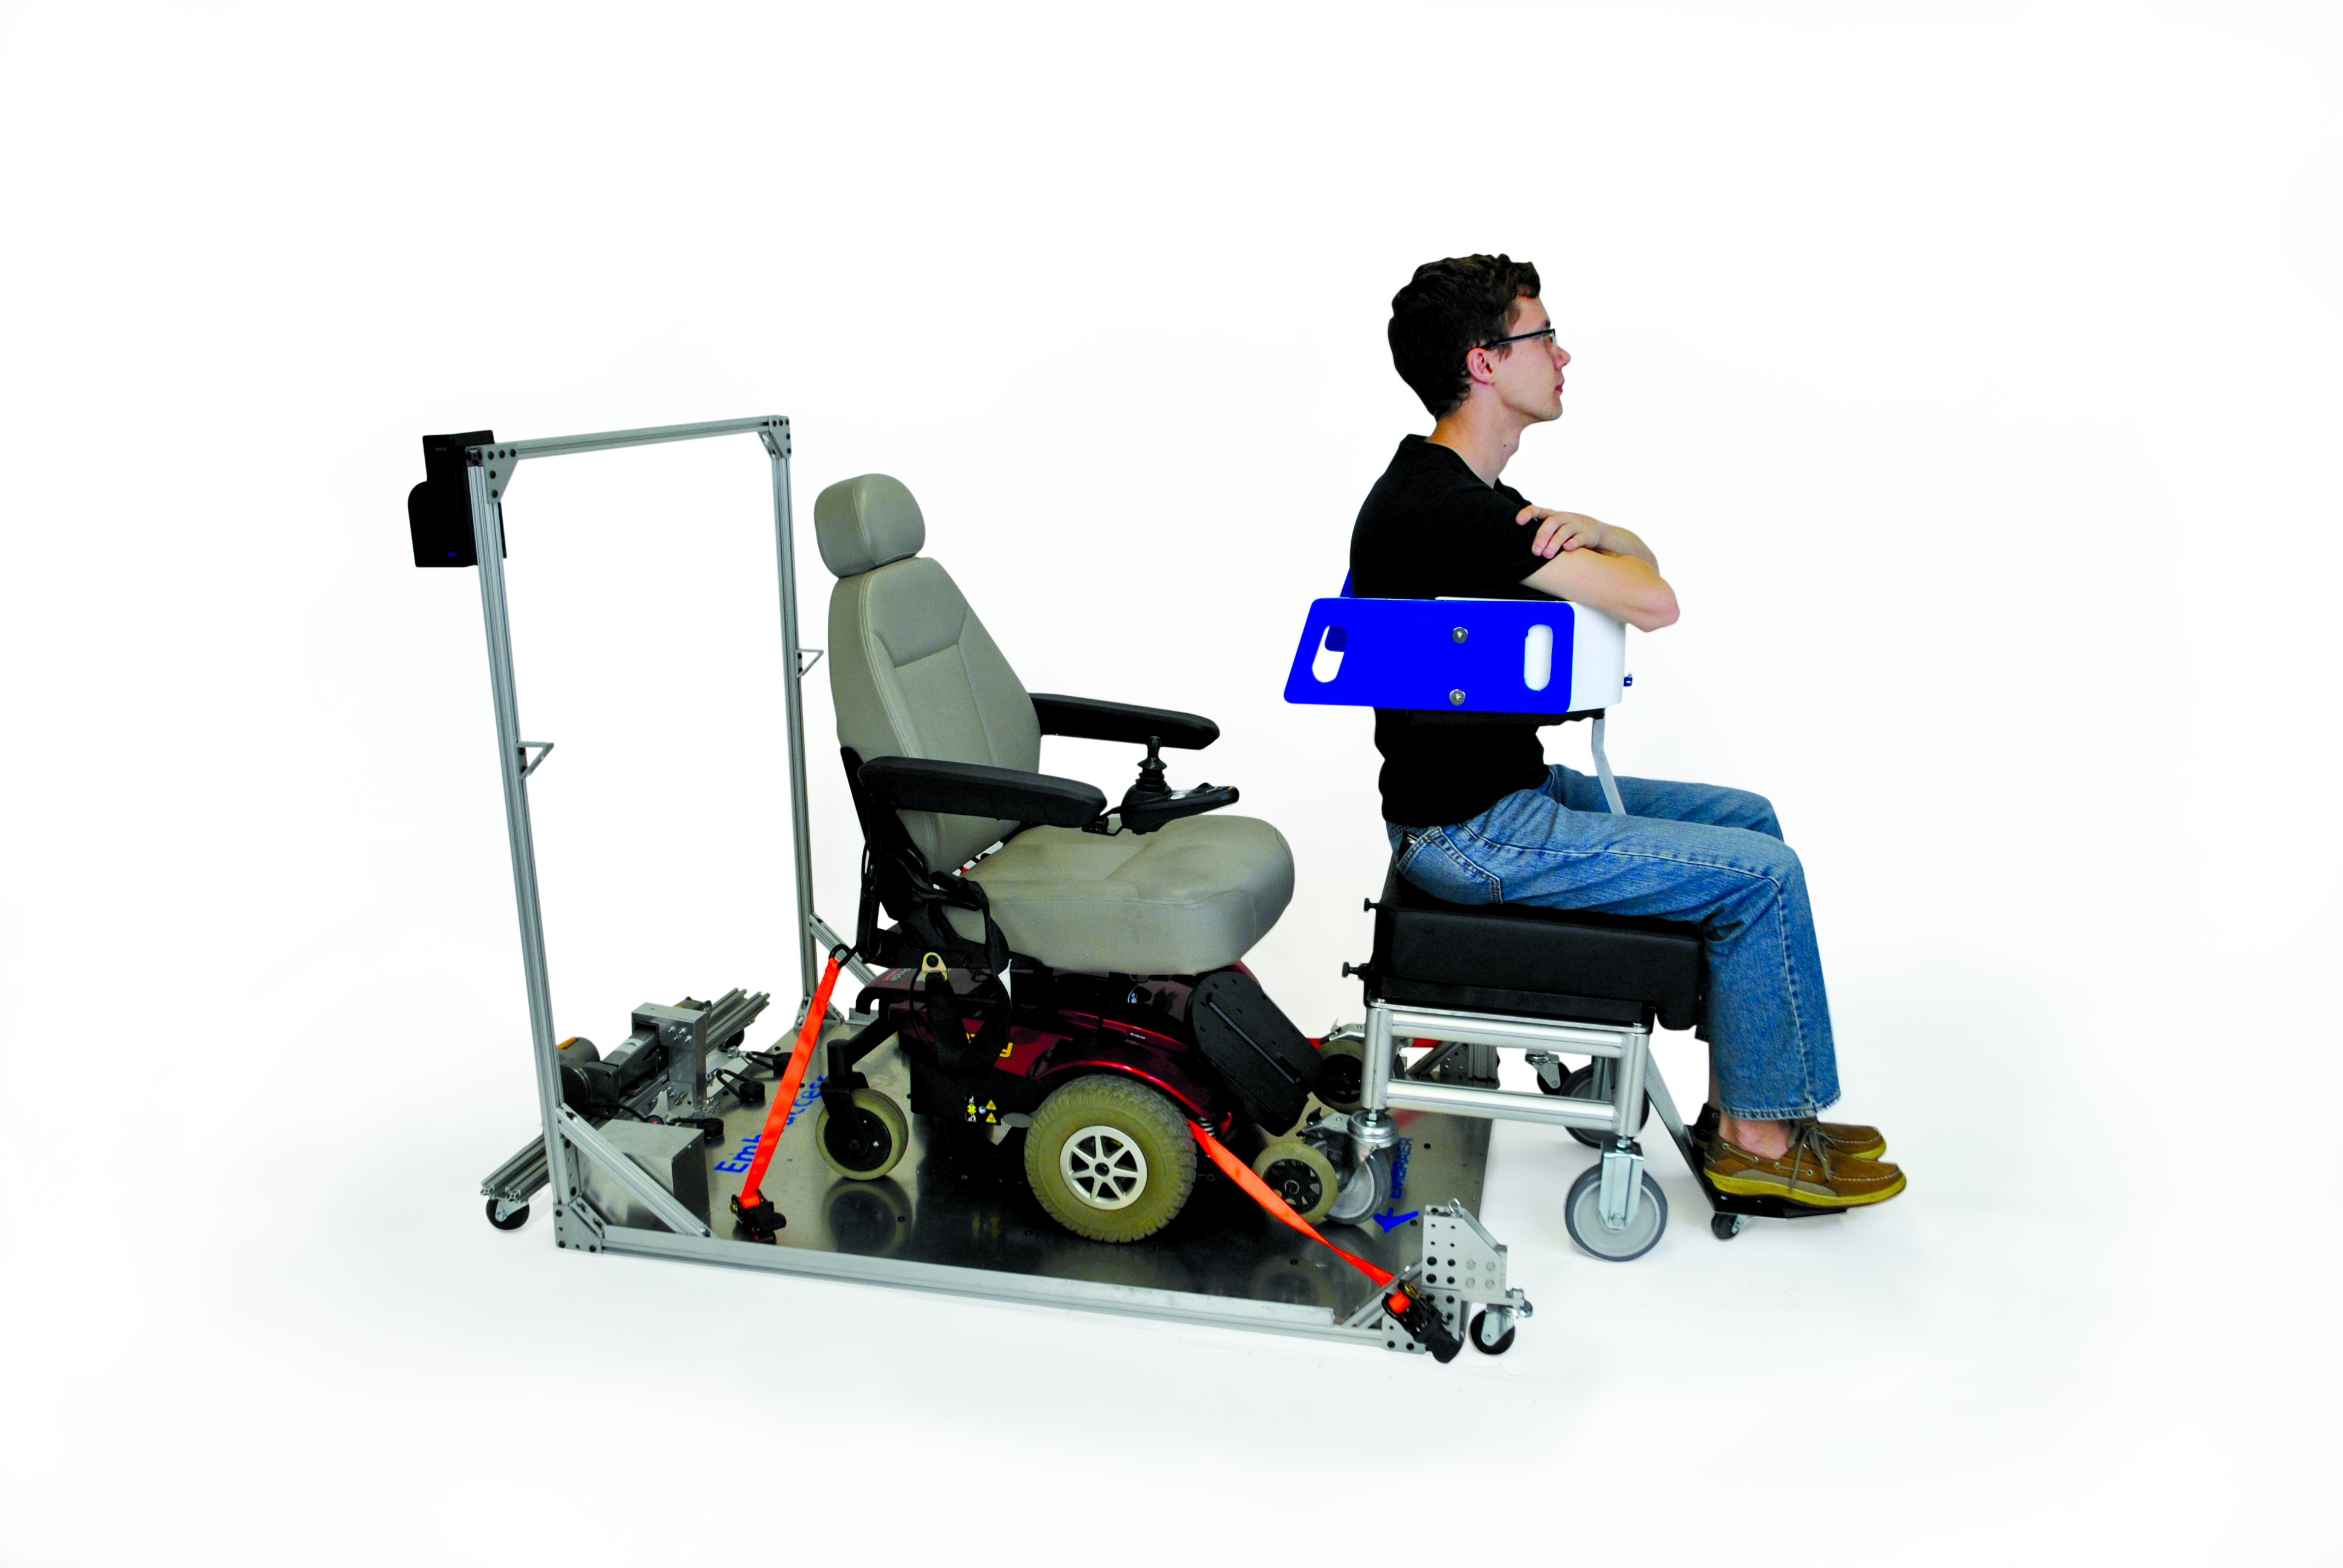
\includegraphics[width=13cm]{images/execsummary.jpg}
\caption{Both products enable a whole new experience for our users.}
\label{fig:exec}
\end{figure}


% add a picture of the whole system

%\section*{Glossary}

%\begin{list}{-}{}

%\end{list}

% Set up the Glossary. The template is looking for a file called
% "glossaryterms.tex" with glossary terms and definitions.
% You can either edit this file manually or you
% can use the Memoir glossary feature in which you insert items like
%   \glossary{glossary term}{our definition of what the term means}
% wherever you like, as you write your documentation.
% When you run the report through Latex, it will create a ".glo" file like
% "OurFallDocument.glo" which you can edit to create the file "glossaryterms.tex"
% There is also perl script I made which will do the formatting for you. 
%  perl Glo2Tex OurFallDocument.glo > glossaryterms.tex

\newpage
\section{Glossary}
%\addcontentsline{toc}{section}{Glossary}
\label{sec-glossary}
\begin{description}
  \item  \textbf{ADA:} Americans with Disabilities Act; one of America's most comprehensive pieces of civil rights legislation that prohibits discrimination against and guarantees people with disabilities have the same opportunities as everyone else to participate in the mainstream of American life.
  \item \textbf{ANAC:} Agencia Nacional de Aviação Civil – Brazilian National Agency of Civil Aviation
  \item  \textbf{Assistive Technology:} Assistive, adaptive, and rehabilitative devices for people with disabilities; promotes greater independence by enabling people to perform tasks that they were formerly unable to accomplish, or had great difficulty accomplishing.
  \item  \textbf{Benchmarking:} A standard by which something can be measured or judged.
  \item \textbf{Control:} The power to influence or direct either people's behavior or the course of events.
  \item \textbf{Dark Horse Prototype:} A device created during the winter quarter of ME310 that was ruled out in the fall quarter or undiscovered due to being “too risky” or “to difficult to complete”; emphasizes creative out-of-the-box thinking and exploring all of the design space for the project. 
  \item \textbf{Disability:} A physical or mental condition that limits a person's movements, senses, or activities.
  \item \textbf{EXPE:} The Stanford design fair that is held every year at the beginning of June. During this fair, all ME 310 teams present the work they have done throughout the year and show their final prototype.
  \item \textbf{FAA:} Federal Aviation Administration; United States national aviation authority whose mission is to provide the safest, most efficient aerospace system in the world, oversees all aspects of American civil aviation.
  \item \textbf{Independence:} Freedom from outside control or support.
  \item \textbf{Limited Mobility:} Mobility impairment may be caused by a number of factors, such as disease, an accident, or a congenital disorder and may be the result from neuro-muscular or orthopedic impairments. It may include conditions such as spinal cord injury, paralysis, muscular dystrophy and cerebral palsy. It may be combined with other problems as well (i.e. brain injury, learning disability, hearing or visual impairment).
  \item \textbf{Needfinding:} Discovering opportunities by recognizing the gaps in the system or the needs.
  \item \textbf{Non-Discriminatory:} Fairness in treating people without prejudice.
  \item \textbf{Pain Points:} A level of difficulty sufficient to motivate someone to seek a solution or an alternative; a problem or difficulty.
  \item \textbf{Perspective:} A particular attitude toward or way of regarding something; a point of view.
  \item \textbf{Self-Image:} The idea one has of one's abilities, appearance, and personality   % input the list "glossaryterms.tex"
\end{description}

%%%%%% Example of an optionally printed "remark"
%\begin{remark}
%\color{blue}
%It's a sign of a successful team that the glossary becomes extensive. Define any non-obvious or invented terms. For %example, if you reference something by an acronym, that might be a glossary term. Teams also coin terms to describe %design features. Define such terms here.  Don't define obvious stuff (axle, keyboard).  

%See comments in me310report.tex if you want to generate a glossary semi-automatically from tagged keywords.
%\normalcolor
%\end{remark}

%%%%%%%%%%%%%%%%%%%%%%%%
% TOC and LOF are automatically generated -- Note that sometimes have to "compile" Latex THREE
% times to update the main .aux files, the TOC etc. files, and finally the PDF output with all changes
% propagated to the printout.
% Make Table of Contents title smaller than a normal Chapter heading:
\renewcommand{\chaptitlefont}{\normalfont\Large\bfseries}
\newpage
\tableofcontents %asterisk to prevent it from getting a number

% Optional Lists of Figures and Tables:
\newpage
\listoffigures  %Note that for this you probably want to add the [short-headings] to captions.
%\listoftables  %I decided to omit the LOT in this example.

%Back to normal size for subsequent sections
\renewcommand{\chaptitlefont}{\normalfont\Huge\bfseries}
%%%%%%%%%%%%%%%%%%%%%%%%




%%%%%%%%%%%%%%%%%%%%%%%%%%%%%%%%
%% On to the main sections....  Just comment out the \input{} line
%% for any chapters that aren't ready yet.

%%%%%%%%%%%%%%%%%%%%%%%%%%%%%%%%
\include{Context}   %Your team, the corporate partner, the project background


%%%%%%%%%%%%%%%%%%%%%%%%%%%%%%%%
% Design Development 
\chapter{Design Development}

Tasked with creating the future of flying for disabled passengers, we carried out process-centric and product-centric needfinding and benchmarking to understand our design space. The insights garnered from these explorations led us to the following key insights which are detailed further in Appendix C.  These insights led us to finally focus on both what happens to the passenger and what happens to his/her wheelchair. The following section is here to show the path our team took to get to this design choice.

\section{User needfinding}
Fall quarter was spent primarily focused on needfinding and benchmarking (see Appendix A) in order to get a firm grasp of the problem we were trying to solving. Given that ``redesigning the flying experience for people with reduced mobility" is a huge design space with a great number of possible users, we used our findings to further develop our understanding of the user segment with the biggest need as well as their specific burning need. After looking at countless available products and interviewing a myriad of different users, we decided to focus on wheelchair users as our target user. 

Throughout our interviews we heard many horror stories about mobility in the cabin and how it affected how wheelchair users prepare for their flights (i.e. ensuring they won't have to use the restroom), how they choose to situate themselves during flight (i.e. choosing to sit in the window seat so they won't be in anyone's way) or whether they even choose to fly. Our final ``experience" prototype for Fall Quarter involved the idea of having seats on rails that would automatically adjust width when a person needed to enter or exit a row. This way, the wheelchair user would have more room to get into their seat and would also be able to choose the seat they wanted because the row would shift when someone else needed to get out, freeing the wheelchair user of the guilt of being in the way. This design addressed painpoints we all encounter while flying (moving in a constrained space) yet would significantly improve the experience for our target user. \\

When we started Winter Quarter we came in with a brand new prospective on the project given that we had just acquired 3 new team members. In order to get the most out of it, we started the quarter by multiple brainstorming sessions in order to identify what were the elements of the aircraft we could change to most improve the travel experience for a wheelchair user- the user we had decided to focus on. 

Through these brainstorming sessions we wanted to understand our design space and its limitations. We also wanted to build a strong relationship with our global partners in Brazil and agreed to meet them on Skype at least once a week and share our common work via a Podio web platform. This helped us keep our teams organized ourselves and aware of the other team's progress and allowed us to tackle and learn about different issues during two big steps in our design development: the dark horse and functional prototypes. 

\section{Dark horse}

\subsection{Introduction}
Winter quarter began with the first of three prototyping missions, Dark Horse.  Named after the horse racing term, this prototyping mission fosters the unimaginable and impossible; improbable solutions to the presented problem from Embraer.  The mission called for the brainstorming of out-of-the-box ideas and the  creation of a physical prototype for this seemimngly implausible solutions.  The learning that occurs from the mission is more important in comparison to the actual building process and it is intended to guide the team toward their final vision. 

\subsection{Benchmarking}
During our interviews and needfinding research, we realized carry-on luggage was a huge concern. Currently, luggage is stored in a very burdensome and unintuitive way and with our prototype we sought out to redesign the carry-on luggage experience. 
Our users have voiced their concerns about not being able to store/reach their luggage as well as the panic they feel when they are not aware of where their belongings are being stored. Our team looked at a couple of different designs out there that use the vertical space within the airplane in a different manner to accommodate both people and luggage in a more user friendly way. 

\begin{figure}[h]
  \centering
     \includegraphics[width=7cm]{images/luggage_trays.png}
   \caption{Design that allows for easier luggage storage for all passengers Source: http://www.gizmag.com/future-of-air-travel-comfortable-seating/17751/}
  \label{fig:luggage_trays.png}
\end{figure}  

The design shown in Figure \ref{fig:luggage_trays.png} displays a cabin layout where consecutive rows of seats are on different levels, allowing passengers to store their luggage behind their tray but under the seat of the person in front of them. This design puts luggage at the ideal height for both standing and sitting passengers as depicted by the image in Figure \ref{fig:correct_height.png}, a standard design rule for accessibility and mobility.  

\begin{figure}[h]
  \centering
     \includegraphics[width=7cm]{images/correct_height.png}
   \caption{Ideal height for reaching objects for both sitting and standing passengers. Source: https://law.resource.org/pub/nz/ibr/nzs.4121.2001.svg.html}
  \label{fig:correct_height.png}
\end{figure} 

Another design solution we explored was actually having two seats on top of each other as shown in Figure \ref{fig:vertical_with_luggage.jpg}. This design opens up the area under the stairs for luggage storage, which could also include a passenger’s wheelchair, allowing for a less stressful flying experience for handicapped users. The bed next to the seat could also be used to provide passengers flying with toddlers with extra room to put them in so that they do not have to sit on their lap throughout the whole flight. 

\begin{figure}[h]
  \centering
     \includegraphics[width=7cm]{images/vertical_with_luggage.jpg}
   \caption{Vertical cabin configuration with luggage storage} % Source: http://www.boston.com/business/articles/2009/06/15/taking_airline_seat_configurations_vertical}
  \label{fig:vertical_with_luggage.jpg}
\end{figure} 

This benchmarking really brought to light the lack on control disabled passengers feel over their belongings. Since they already suffer from mobility constraints, they are not able to fully control where their belongings are stored which causes a huge amount of anxiety. We realized later on that this anxiety was only increased when the object in question wasn't just a bag but rather a mobility device. 


Another main concern for our user was the actual transfer process and how they would get from an aisle chair to their seat. We know that today people can use transfer boards, they can be carried by someone else or, if they are strong enough, they can attempt to transfer themselves(although the limited space in the cabin makes this virtually  impossible). We found that there are some products on the market utilized in analogous situations that could make the transfer experience better, such as the “harness” shown in Figure \ref{fig:harness.jpg} or the walker in Figure \ref{fig:walker.jpg}. We believed that the walker would be an interesting solution if we were able to add mechanisms that would lower the bar supporting the person’s weight to get it closer to the seat and that would swing the blue supports open such that the person would come in contact with the chair. In the end, we decided to opt for a more futuristic vision and decided to widen the airplane aisle and get rid of the transfer all together. 

\begin{figure}[h]
  \centering
     \includegraphics[scale=0.3]{images/harness.jpg}
   \caption{Harness used to get disabled out of the bath.}% Source: http://www.handimove.com/en/products/bath-seat-pvc/}
  \label{fig:harness.jpg}
\end{figure} 


\begin{figure}[h]
  \centering
     \includegraphics[scale=0.5]{images/walker.jpg}
   \caption{Walker that could be adapted to become a better aisle chair.}% Source: http://mobilityexpress.com/Sara-Stedy-Seated-Transfer-Device_1154.htm}
  \label{fig:walker.jpg}
\end{figure} 

\subsection{Description of the prototype}
Currently, people with reduced mobility have to first transfer from their own wheelchair to an uncomfortable and narrow aisle wheelchair. Once boarding starts, the user is brought to his/her seat by a flight attendant or an airline employee and is then transferred to his/her seat, usually by being carried over their shoulders. This process is long, dehumazing and it deprives them from their independence. Since the boarding process is such a pain point for our users, we decided to tackle this problem to improve their experience and give them more independence. Our team thought that if we could enable people with reduced mobility to enter the aircraft with their own wheelchair and then give them the possibility to transfer themselves from their wheelchair to their seat without someone else helping them it would considerably improve their experience.
\\

%During the boarding process the two steps that are critical for our users are :

 %\begin{easylist}[itemize]

%& First, the access to their seats. 

%& Second, the luggage storage. People with reduced mobility frequently cannot access the luggage compartment because it is too high, so our team thought that if we could imagine a system that makes the luggage compartment go up and down by just pressing a button it would also contribute to make the flight experience better for people with reduced mobility.

%\end{easylist}


\textbf{Helping our user access his/her seat :}

Our objective was to enable passengers to enter the aircraft with their own wheelchair and to do so we had to figure out a way to make the aisle wider. Initially we did not want to take into account the constraint of keeping the number of seats in the aircraft the same so we imagined a new cabin layout for boarding. The idea was to have the aisle seats on rails so that they could be moved and lined up with the window seats as shown in Figure \ref{fig:first_new_cabin_layout} . 

\begin{figure}[h]
  \centering
     \includegraphics[width=7cm]{images/first_new_cabin_layout.png}
   \caption{Our first new cabin layout for boarding the plane}
  \label{fig:first_new_cabin_layout}
\end{figure} 

With this system, all the seats would be lined up on each side of the plane and the aisle during the boarding process would therefore be three times bigger than during the flight, giving people with reduced mobility the ability to enter the aircraft with their own wheelchair since the average width of a wheelchair (30’’ as shown in Figure \ref{fig:wheelchair_dimensions} ), would now fit down the bigger aisle. 

\begin{figure}[h]
  \centering
     \includegraphics[scale=1]{images/wheelchair_dimensions.png}
   \caption{Standard wheelchair dimensions}
  \label{fig:wheelchair_dimensions}
\end{figure}

But we realized that with this system it would be impossible to keep the total number of passengers on board the aircraft the same since the proposed boarding layout required too much space per seat. 

Therefore, we thought of a second cabin layout for the boarding process which would also make the aisle wider but in a more reasonable way. We looked at the dimensions of a standard Embraer plane (Figure \ref{fig:embraer_plane} ) and found out that if we were able to angle the rows by 46.2° (see Figure \ref{fig:angled_seats}) from their current position we could make the aisle wide enough (42.87’’) to enable our passengers to reach their seats in their own wheelchair while still keeping the total number of seats the same.

\begin{figure}[h]
  \centering
     \includegraphics[width=7cm]{images/embraer_plane.png}
   \caption{Standard Embraer plane cabin layout}
  \label{fig:embraer_plane}
\end{figure}

Our concept was to initially have all of the rows of the plane linked to a mechanism that would rotate the seats before the boarding process, making a wider aisle for passengers. Passengers with reduced mobility who have reached their seats with their own wheelchair would be able to transfer themselves  to their plane seats. 
\begin{figure}[h]
  \centering
     \includegraphics[width=7cm]{images/angled_seats.png}
   \caption{New cabin layout with angled seats for boarding}
  \label{fig:angled_seats}
\end{figure}

Once the passengers are all seated (potentially while the aircraft is taxiing towards the runway) the seats would go back to the standard non-angled cabin configuration for take-off and would remain in that state for the duration of the flight. When the plane stops at the gate and is ready for passengers to disembark, the seats would be angled again and flight attendants would bring passengers with reduced mobility their own wheelchair. This configuration would completely remove the need for an aisle wheelchair.\\ 


%\textbf{2. Helping our user accessing the luggage compartment :}

%We found out that accessing the seat is not the only problem disabled people are confronted with: they also have a big issue when they want to store their personal items in the luggage compartment. In order to fix this, our team designed a luggage compartment that can go up and down on demand, controlled by our user pressing a button (Figure \ref{fig:embraer_plane}).

%\begin{figure}[h]
%  \centering
%     \includegraphics[width=7cm]{images/20140130_170818.jpg}
%  \caption{Our luggage compartment which is accessible on demand by pressing a button}
%  \label{fig:our_luggage_compartment}
%\end{figure}

%In order to build this system we designed a mechanism made of rope and pulleys that is inspired from systems used to stabilize cameras that are mounted on drones and model aircraft. While piloting the system that causes the camera to move, the device has to remain stable. This mechanism avoids the creation of moments that could cause the ropes to tangle and knot. For our system we wanted to have a luggage compartment that does not experience torques and that can come up and down in the most smooth and stable way.

\subsection{Learnings}
Several classmates and peers were users for this prototype and provided the majority of our learnings.  However, some of the learnings came directly from team observations during user testing. 
\\

\textbf{Reconfiguration:}
\begin{easylist}[itemize]
	& Our testing revealed that the users were concerned about what would happen to their feet during the transformation of angled seating to the regular configuration and vice versa.  Some users suggested the addition of a footrest.  But where would the ideal location be? This revelation is very important to our target users because some of them do not have the ability to move their legs out of the way or to move with the chair.  This would also mean they would have to manually put their feet on a footrest, and the ideal position of the footrest would need to be designed to help the target users have a better experience.
	& A single, continuous rotation mechanism would be better than multiple discrete ones for all passengers.  The users commented that the mechanism should be similar to the movement of a car seat because it so slow it is barely felt. In addition, the window seat felt like it experienced less movement partly because the displacement was smaller than for the aisle seat.  This is important due to the benchmarking findings of last quarter that showed that the target users preferred the window seat over the aisle seat. 
	& Passengers would be able to board faster due to a wider aisle that allows for easier maneuvering of the cabin space.  The wider aisle would allow for a double line of traffic to head down the aisle instead of one line. 
	& The wider aisle would allow for a wheelchair to be able to maneuver down the aisle to the seat.  The wheelchair would have space on both sides as it moves down the aisle to allow for a comfortable fit.  It would be easier for a mobility challenged passenger to get into the aisle seat but they may need a handle to access the window. 
	& The legroom is the limiting factor with the reconfiguration.  When the seats are in the angled arrangement, the window seats have less legroom than in the normal configuration.  The angle of the seats would need to be reconfigured to allow for a smaller angle with more legroom but still create a wider aisle with plenty of tolerance for a wheelchair. However, it was noted that it is easier to board and deboard with angled seats.  Thus, angled seats would be the preferred configuration for boarding and disembarking from the plane. 
	& It may be possible to achieve the desired effect by only rotating several of the aisle seats, allowing increased access to those seats specifically.

\end{easylist}


%\textbf{Luggage storage:}
%\begin{easylist}[itemize]
%	& The luggage bin needs to move with the seats into the angled configurations. With the bins situated parallel to the normal cabin configuration when the seats are angled, it is difficult to load the luggage into the bin without awkward movements. 
%	& The luggage bin should be lowered to arm level instead of head or face level.  Users felt claustrophobic when the bin was at head level due to the reduction in vision. The bin was in the line of sight which made it uncomfortable and a very closed-off space.  
%	& The bin should have a door and have a slightly steeper angle or have a lip. Luggage moves during flight due to turbulence and shifting due flight. This would prevent luggage falling out on the passengers or items being broken. 
%	& A more rigid lowering mechanism needs to be used instead of the string and rope mechanism that was used during prototyping.  Users did not feel that the bin was stable and looked scared as it was lowered down.  They feared the bin might move during lowering, raising, or turbulence causing it to hit them or bring their belongings.  
%	& More research for optimal lowering position needs to be conducted.  The position that we prototyped did not receive good feedback from the users.  Therefore, several iterations need to be performed to see what would be best for our target users and other passengers
%	& Most of the users wanted to store luggage before they sat in their seat.  The orientation of the bin and the height of the bin makes this a very awkward and uncomfortable task.  When the users sat with their luggage, they felt that they were crowded and did not know what to do with the luggage until the bin was available.  The mechanism to raise and lower the bin needs to be fast and stable to allow for ease of access to the seat and aisle depending on the activity.
%\end{easylist}

\section{Going Back to The Need}

Following the wrap up of our prototypes, the team decided to take a step back to figure out if we were truly solving the burning need. We analyzed all of our prototypes up to this point and saw an overarching theme we were trying to address: giving our users their independence back. With independence as our umbrella, our team looked at the whole flying experience piece by piece (see Appendix B), with the purpose of identifying the points at which independence truly breaks down. 

We went back to our needfinding from fall quarter, sent surveys to both old and new contacts and carried out more interviews. All of these allowed us to confirm that mobility within the cabin is, in fact, a huge issue. However, this new information also brought to light a burning need we had initially discarded fall quarter - wheelchair storage. Furthermore, both of these needs stem from the same procedure the wheelchair user is forced to go through: that of giving up his/her wheelchair. \\

\textbf{The Problem}

Imagine you are a wheelchair user. You arrive at your gate, ready to board your plane, and are told you need to hand over your wheelchair for storage in the cargo hold. At this point, you ask yourself two questions: 
\begin{enumerate}
	\item How will you move now that you don't have your mobility device? 
	\item Will your mobility device arrive safe and sound at your destination?
\end{enumerate}
The following sections will detail the user quotes and research that led us to choosing both of these directions.  
\\

\textbf{Mobility In the Cabin}

In order to confirm the need for improving mobility inside the cabin, we asked our contacts to fill out a survey that would give us a better idea of what exactly would be the most helpful for them. The full survey responses can be found in Appendix D.
 
When asked about the prospect of having an ``on demand"  powered aisle chair, users were keen on the independence it would provide as it would allow them to ``board the plane at [their] own pace and go to the restroom when [they] please." One of our respondants stated that such a device would allow them to ``feel like a passenger for a change and not a sack of coffee beans". This quote clearly depicts the struggle users currently go through when they give up their mobility device and along with it, their independence.

Our team assumed that having such a chair would be a great improvement to the experience yet we could not figure out if the chair had to be completely autonomous and show up on demand or if a flight attendant could bring it to the user. What we found is that users would much rather have automated systems than feel the guilt of inconveniencing someone else to do something for them, even if it only meant they had to bring them a chair just like they bring any passenger a drink or snack. 

Finally, we decided to delve deeper into the transfer process. One of our interviewees, Scott Rains, had told us about a friend who was injured as he was being transferred from the aisle chair into his airplane seat. The airport personnel did not lift him up high enough and his bottom was hit against the armrest. Given that wheelchair users have thinner and more sensitive skin in this area, this caused him lots of pain and even resulted in 3 weeks spent at the hospital. While injuries are not the norm, it is a very dehumanizing and undignified experience, just as Esther Appleyard-Fox states in her tweet in Figure \ref{fig:MobilityTweet.png}. 


\begin{figure}[h]
  \centering
     \includegraphics[width=9cm]{images/MobilityTweet.png}
   \caption{Tweet from Esther Appleyard-Fox explaining how she feels when she is transferred when she flies. }
  \label{fig:MobilityTweet.png}
\end{figure}


\textbf{Wheelchair Storage}

As we were looking for more data to substantiate our claim that mobility in the cabin was, in fact, the problem to solve, we stumbled upon another huge problem. During our interview with Aubrie Lee, a student in Product Design at Stanford University who is also a wheelchair user, she mentioned that while mobility inside the cabin is a problem, it is such a short part of her experience that she hardly remembers it as being painful. Part of this is due to the fact that when she travels with her dad he carries her down the aisle which can be more a comforting bonding moment than dehumanizing. However, she emphasized that``the most emotional part of [her] flying experience is having to give up [her] chair and waiting for them to give it back." For her, giving up her chair is ``a huge source of anxiety - as soon as it is out of [her] sight, [she doesn't] know where it is", whether it is going to come back to her unharmed or whether it is even going to make it to her destination. 

In order to understand what can happen to a mobility device on during its transfer to the plane and once in flight, we interviewed an Air France employee working at Toulouse-Balgnac airport (France). All the details form this interview are in Appendix E. It shows how airlines handle wheelchairs from the jetway to the cargo hold and gives some insight on the type of damage that can occur.

A study by Trailblazers\footnote{http://www.mdctrailblazers.org/assets/0000/8262/Trailblazers$\_$AirlineReport$\_$WEB.pdf}, a group of disabled campaigners across the UK who tackle social issues affecting young disabled people, shows that 60\% of wheelchairs are damaged when traveling with an airline. As David Gillon says in Figure \ref{fig:60percenttweet} below, we must do better. 


\begin{figure}[h]
  \centering
     \includegraphics[width=9cm]{images/60percenttweet.png}
   \caption{Tweet from David Gillon on Trailblazers study that shows 60\% of wheelchairs are broken in airline travel. }
  \label{fig:60percenttweet}
\end{figure}

\begin{figure}[h]
  \centering
     \includegraphics[width=5cm]{images/wheelchairstory.png}
   \caption{Anecdote from a Trailblazer that had her wheelchair broken during flight.}
  \label{fig:wheelchairstory.png}
\end{figure}

Stories like the one shown in Figure \ref{fig:wheelchairstory.png} are not uncommon, with wheelchairs ending up like the one in Figure \ref{fig:brokenwheelchair.png} due to airport personnel attempting to dismantle it or from the wheelchair moving around in the cargo hold. 


\begin{figure}[h]
  \centering
     \includegraphics[width=7cm]{images/brokenwheelchair.png}
   \caption{Picture of a broken wheelchair after a flight.}
  \label{fig:brokenwheelchair.png}
\end{figure}

There are also instances of the wheelchair not even making it to the destination, just like what happened to Josie shown in Figure \ref{fig:leftwheelchair.png}. 

\begin{figure}[h]
  \centering
     \includegraphics[width=9cm]{images/leftwheelchair.png}
   \caption{Tweet from Josie Verguese about her experience when her wheelchair did not make it to her destination.}
  \label{fig:leftwheelchair.png}
\end{figure}

Now to put this into perspective, imagine that you are a wheelchair user and you rely on your mobility device for you independence. This wheelchair isn't just an object, it is your legs, your independence, part of who you are. As Aubrie stated  my wheelchair``is in limbo between being a physical object and half of me." Now imagine that after your flight, you no longer have the ability to move. This is a HUGE problem for our users, one we need to focus on. \\
\\

 Through  the user interviews, surveys and research depicted above, we have proven to ourselves, our advisors and our users that these are the 2 most compelling needs we need to address for our users and we decided to focus on both for the Functional Prototype. 


\section{Functional Prototype}
The final prototyping mission during Winter Quarter was the Functional Prototype in which we had to create a working prototype with system integrations using materials that could be present in a final vision. The functional mission leads the team into the Spring Quarter by aiding in the finalization of the vision and creating an actionable direction.  To find the direction and the vision, more needfinding might have to take place to confirm a need and verify the thinking and decisions of the team. The Functional mission serves as the stepping point from iterative prototyping missions to the iterative final product mission.

\subsection{Wheelchair Storage Benchmarking}
Before prototyping our first wheelchair storage device we executed a larger search both for existing wheelchair storage and protection devices as well as methods for securing wheelchairs. We found several relevant patents for protection devices as well as regulations for securement, relating primarily to bus travel. \\

\noindent\textbf{Securement}\\
The United States Department of Transportation's Federal Motor Carrier Safety Administration publishes a wide array of regulations. Included amongst the regulations governing school bus safety, Federal Motor Vehicle Safety Standards \textsection 571.222 \cite{fmvs222}, are a number of requirements for how wheelchairs must be secured while in transit. The section requires that the wheelchair is secured in four locations, with an additional three point mounting required to secure the student. Similar topics are covered in further regulations, such as Title 49 \textsection 38.23 \cite{ecfr}. Figure \ref{fig:tie-down} demonstrates the general setup. \\

\begin{figure}[h]
  \centering
     \includegraphics[width=7cm]{images/wc_van.jpg}
   \caption{Wheelchair tie-down setup for van travel}
  \label{fig:tie-down}
\end{figure}

\noindent\textbf{Storage}\\
A group at Utah State University performed market research \cite{USU_survey} and designed a prototype wheelchair storage container, determining that over 50\% of their surveyed users might be or would be interested in their device. A drawing of their box, which provides several securement methods for wheelchairs and other objects, can be seen in Figure \ref{fig:USU_box}; more information is in US Patent application 12/142,662.\cite{USU_patent}

\begin{figure}[h]
  \centering
     \includegraphics[width=7cm]{images/USU_box.png}
   \caption{Storage container}
  \label{fig:USU_box}
\end{figure}


\subsection{Wheelchair Storage Description}

As our last round of needfinding and research had brought to light the importance of wheelchair storage, the Stanford team decided to prototype the first version of what a wheelchair storage device could look like. This first prototype, shown in 
Figure \ref{fig:wheelchairprototype1.png}, focused on having a rigid floor to distribute the weight of the wheelchair as well as a place to attach the hooks that would secure the wheelchair down. It had rigid walls that would serve to protect the wheelchair (as if it were a box) that were also hinged at the side so they could be moved out of the way as the handler was tying down the wheelchair. We opted to use the straps and hooks mechanism that people are already familiar with from buses and trains to create a sense of trust and security. 

\begin{figure}[h]
  \centering
     \includegraphics[width=7cm]{images/wheelchairprototype1.png}
   \caption{First prototype of wheelchair storage device.}
  \label{fig:wheelchairprototype1.png}
\end{figure}

Since many of the stories we encountered about wheelchairs being damaged involved airport personnel attempting to disasemble them or handling them poorly, we wanted the wheelchair owner to be present during the securing process, just like they are on a bus or train. This way, the wheelchair user could help the airport personnel speed up the process by providing information about their specific wheelchair and how it should be secured as well as ensure that the airport personnel is not accidentally mishandling their mobility device. At the end of the securing procedure, the container is to be closed up, giving the user satisfaction in knowing that their wheelchair is secure and will arrive safely at their destination. 
 
Because the wheelchair user is present while their wheelchair is secured, we must also enable an easy transfer from their personal wheelchair onto the aisle chair. As shown in the rendering  Figure \ref{fig:storagetransfer.png}, right now this is accomplished by bringing the transfer chair close to the passenger's chair that is already secured. This further explains our use of hinged walls and puts a hard constraint on our system- in order for the wheelchair user to be able to easily transfer once their wheelchair is secured, there must be a way to ``remove'' all walls during securing and ``reappear'' them once the wheelchair is stored for the wheelchair to be protected.

\begin{figure}[h]
  \centering
     \includegraphics[width=7cm]{images/storagetransfer.png}
   \caption{Rendering of wheelchair and aisle chair side by side once wheelchair has been secured.}
  \label{fig:storagetransfer.png}
\end{figure}

While there are certain hard constraints that were not met with this protoype, we are keeping them in mind and will insitute them in future iterations. We know the container must protect the wheelchair but also fit through the door to the cargo hold as well as fit inside the cargo hold. It needs to be movable, as the wheelchair storage container must travel from the jetway down into the cargo hold. This product must help the luggage handler create a connection with the wheelchair user and gain empathy for the importance of the mobility device that is in their hands; the more important they know it is, the better they will treat it. Finally, the storage device must be lightweight as this is of utmost importance to Embraer and the airlines they serve.

\subsection{Wheelchair Storage Learnings \& Next Steps}

From our first prototype we were able to learn a myriad of things. Primarily, we realized that using a mechanism that wheelchair users are already familiar with is a huge plus; it provides them with a feeling of trust and security that their wheelchair will not be damaged throughout their flight. Thus, we suceeded at providing the user peace of mind with this device. However, we realized it is pretty difficult to line the chair up in the correct configuration in between the protruding hooks that strap the wheelchair to the platform and thus it would be best to have the hooks be flush against the top of the base so they didn't get in the way of the wheelchair manuevering.
We had several users go through the process of securing the wheelchair and found that having simple straps and hooks can be confusing and time consuming. Thus, it is best to have retractable hooks that come out of the base so that the tension is automatically set, making the job of the securer much easier. 

For a process that takes place prior to a flight, time efficiency is extremely important. Airport personnel are very crunched for time as they cannot afford to have any process delay the flight and push their schedules back. This means having very clear instructions for both the wheelchair user as to what's expected of them, where to park and how the process will unfold, as well as for the person securing the wheelchair. For the wheelchair user, we are thinking of ways to transfer this imformation prior to their flight, knowing that most disabled passengers keenly do their research before flying. Having a video that shows the whole process would allow the wheelchair user to be prepared to tell the securer exactly what the right attachment points are and how to best secure the wheelchair down. On the other hand, it is important for the securer to know the correct order of the procedure which can be accomplished by numbers next to each hook as shown in Figure \ref{fig:instructionsstorage.png} and simple drawings depicting what's next. 

\begin{figure}[h]
  \centering
     \includegraphics[width=7cm]{images/instructionsstorage.png}
   \caption{Securing the wheelchair}
  \label{fig:instructionsstorage.png}
\end{figure}

Finally, our user testing confirmed our theory that we would need retractable walls. Not only were they necessary for the user to easily transfer onto the aisle chair but they also made the securing process much easier. The back wall, however, was still rigidly attached. This, we found, was not ideal as it made the two hooks in the back extremely hard to reach. With this information in mind, we have been brainstorming different design ideas that would enable for the walls to be completely out of the way during boarding and securing yet would be present during flight to protect the wheelchair from being damaged. We have thought about accordion or telescoping walls as well as having inflatable walls. We really liked the idea of inflatable walls as it provided the wheelchair with protection from damage yet could be blown up to accomodate different types of wheelchair sizes and would be extremely light weight. A preliminary mock up of a possible vision can be seen in Figure \ref{fig:inflatablesrendering.png} With this in mind, we began a feasibility study to understand how possible the use of inflatables would be in the application. 


\begin{figure}[h]
  \centering
     \includegraphics[width=7cm]{images/inflatablesrendering.png}
   \caption{Rendering of a preliminary idea of what an inflatable ``wall'' could be.}
  \label{fig:inflatablesrendering.png}
\end{figure}

%take it from here robbie!

\subsubsection{Inflatable Materials}

In order to test the feasibility of an inflatable device in the cargo hold there were a few problems that needed to be addressed.\\
\noindent\textbf{Pressure}\\
The cargo hold of many planes is not pressurized in order to save on costs. One of our goals was to determine if an inflatable device to protect the wheelchair would pose a problem in low pressure situations. Initially we were unsure as to what the pressure in the cargo hold would be, and as such decided to design for the worst case when the pressure is the same inside the cargo hold as outside. 

It was important to design for this case as regardless of the pressure in the cargo hold, in any emergency situations where the cabin lost power, we would not want any problems to arise in the cargo hold potentially making the situation worse.\\

\noindent\textbf{Temperature}\\
A second potential problem with an inflatable device in the cargo hold is that the luggage does not require the same heating and insulation as passengers. While it may not get as cold as the air outside (approximately -40 C) in normal situations, we must design the device to work reliably even in case of an emergency. \\

\noindent\textbf{Testing}\\
While it may  be possible to test the effects of pressure on an inflatable device without taking it into a plane by increasing the pressure inside the inflatable device (since the pressure differential is the most important aspect to test), its much more difficult to test this pressure differential at a realistic temperature on the ground. Instead we decided it would be best to get an inflatable structure up to approximately the height of a plane and determine what failure modes, if any, would be present. 

In order to do this we attached a fully blown-up arm flotation device to a weather balloon. This balloon was released in order to take the device into the upper atmosphere where it would experience similar conditions to those of an airplane. While it ignores some effects from the natural plane insulation, its a more extreme environment in all cases so its a good measure of feasibility. \\

\noindent\textbf{Results}\\
Unfortunately the barometer which was being used as an altimeter for this experiment failed, and as such we were unable to get reliable altitude data on the flight. However by looking at the videos returned from the launch, and given the group's prior experience with weather balloons, a reasonably reliable estimate of 50,000 - 60,000 ft can be estimated for when the flotation device popped,an altitude which is significantly higher than an Embraer jet flies (37,000 ft maximum). We were able to see small water droplets on the larger weather balloon which froze at high altitudes forming ice crystals.

This experiment showed us that an inflatable solution would in fact be feasible if it was something we wanted to pursue.

\subsubsection{Wheelchair Tracking Concept}

We didn't just want to stop at protecting the wheelchair, we also wanted to give the wheelchair user information regarding their wheelchair. 
We envision a wheelchair tracking system in which each storage container has a unique identifier, such as a QR code, which can be tracked as the container moves from the jetway to the tarmac, into the cargo hold, and then back out again after landing. The identifier can be recognized at a series of checkpoints, which need to consist only of a webcam if a QR code is used. Such a system will provide our users with the peace of mind that their mobility device has not been mistreated or left behind.

\begin{figure}[h!]
  \centering
     \includegraphics[width=12cm]{images/tracking.png}
   \caption{Wheelchair tracking system overview.}
  \label{fig:tracking}
\end{figure}


An important aspect of this system is that it can also help develop empathy on the part of the baggage handlers. Wheelchair users will have the opportunity to tip handlers who've done a good job in managing their mobility device, both providing an incentive for doing a better job while also helping form a closer connection between two people who may never meet face to face.

An overview of the system and one potential user interaction are in Figures \ref{fig:tracking} and \ref{fig:tips}.


\begin{figure}[h]
  \centering
     \includegraphics[width=7cm]{images/tips.png}
   \caption{One possible minimal interface for user interaction with the tracking system.}
  \label{fig:tips}
\end{figure}


\subsection{Transfer mechanism from aisle wheelchair to seat}

Once the problem of wheelchair storage storage is addressed, there is still one that needs to be solve: how do disabled passengers reach their seats once their mobility device is stored in the cargo hold? \\

Our benchmarking and interviews showed us that the transfer is one of the most demeaning moments for the handicapped, so the team focused on making the user more independent while transferring. \\

\subsubsection{Candidates}
The team agreed that the prototype should make the transfers inside the airplane so easy that the person on the aisle wheelchair could make the transfer by himself without major efforts. After a brainstorm, the team had two ideas for making this transfer: a sliding seat and a comb mechanism in which a male/female coupling system would allow the user to be transferred. The former mechanism was chosen because it was simpler to build and lighter, as it did not require a motor to lift the user or a counterweight to stabilize the chair. With that in mind, we benchmarked existing mechanisms that were used to make linear transfers. These mechanisms are listed below: \\

\noindent\emph{Linear Guide}\\
The rails would be installed on the aisle wheelchair and the seat, while the carriage would be installed on the cushion. The cushion would be able to slide from one seat to the other if the seat and the wheelchair were correctly paired.

\begin{figure}[h]
\centering
\includegraphics[width=7cm]{brazil_images/image035.jpg}
\caption{Linear guide} % - http://www.yesillerrulman.com/staf_lsk_ome_lineer_kizakli_araba_ray.html}
\label{fig:linear_guide}
\end{figure}

The negative aspect of the linear guide is that it would require a milimetric precision when pairing the aisle wheelchair with the seat. We found this to be unrealistic, especially when we took in consideration that the solution would not necessarily be automated.\\

\noindent\emph{Conveyor rollers}\\
The mechanism would use the same principles of a conveyor table, where one can move heavy objects by sliding them on top of conveyor rollers. This mechanism would be installed on the seat and the aisle wheelchair, allowing the cushion with the user to slide.

\begin{figure}[h]
\centering
\includegraphics[width=7cm]{brazil_images/image036.jpg}
\caption{Conveyor rollers} % - http://qdtmzdhsb.cn.gongchang.com/product/d27215965.html}
\label{fig:conveyor_rollers}
\end{figure}


\noindent\emph{Caster transfer table}\\
The mechanism would work as the previous one, where the cushion would be able to slide from the aisle wheelchair to the seat, but using caster spheres instead of conveyor rollers. These spheres are lighter than the previous solution and as a result were more appropriate for our design.

\begin{figure}[h]
\centering
\includegraphics[width=7cm]{brazil_images/image037.jpg}
\caption{Ball transfer table}% -  http://www.stackbin.com/categories/ball-transfer-tables/ }
\label{fig:ball_transfer}
\end{figure}

Unfortunately, for our first prototype, we could not find a supplier that could provide the components in time to build the prototype with an affordable cost, so the mechanism with they conveyor roller was chosen. For the final prototype, the team was finally able to get the caster spheres into the device and implement them.

Based on what was discussed above, for the first version, the team decided to implement the seat with conveyor rollers to enable the sliding movement of the seat (Figure \ref{fig:idea_mechanism}). With the same mechanism installed on the aisle wheelchair, one would be able to easily transfer oneself laterally from the aisle wheelchair to the seat and vice versa without major efforts.

\begin{figure}[h]
\centering
\includegraphics[width=7cm]{brazil_images/image038.png}
\caption{Idea of the mechanism}
\label{fig:idea_mechanism}
\end{figure}


\subsubsection{Building our prototype}
In our first attempt to build the prototype (Figure \ref{fig:first_attempt}) the high friction made the sliding movement extremely difficult. The main reason for this failure was that we incorrectly assumed that the aluminum cylinder directly attached to the wooden structure would be enough to make the rolling movement. \\

\begin{figure}[h]
\centering
\includegraphics[width=7cm]{brazil_images/image039.jpg}
\caption{First building attempt}
\label{fig:first_attempt}
\end{figure}


In order to overcome this issue, we added bearings to both ends of the cylinders (Figure \ref{fig:fixing_bearings}). This solved the friction problem, making the whole mechanism work as we had designed it (Figure \ref{fig:final_mechanism}).	


\begin{figure}[h]
\centering
\includegraphics[width=7cm]{brazil_images/image040.jpg}
\caption{Fixing bearings}
\label{fig:fixing_bearings}
\end{figure}


\begin{figure}[h]
\centering
\includegraphics[width=7cm]{brazil_images/image042.jpg}
\caption{Final mechanism}
\label{fig:final_mechanism}
\end{figure}

Next, we tested the sliding mechanism with different types of materials on the cushions base. First we tried adding an adherent surface (rubber) to see how the mechanism would slide. We noticed that it was quite hard to overcome the static friction. Afterwards we tried adding a semi-rigid plastic base. Although the transfer was quite easy, one could feel the cylinders while sliding. As a result, we chose to use a hard flat base under the cushion to make it slide smoothly.   \\


\subsubsection{Learnings}

We tested our mechanism with a number of able-bodied users as we were not yet confident that it was safe enough for a disabled person to use it. We learned alot from these testing sessions and it thanks to these learnings that we were able to create a product that could be safely used by a disabled person.

\begin{itemize}
	\item The friction between the aluminum cylinder and the wood is too intense for a user to transfer from one seat to another.
	\item The space between the cushion and the mechanism must be considered to avoid increasing the friction and the looseness of the cushion (due to a rotating movement).
	\item Cushion must be firm enough so that the user does not feel the cylinders and to allow proper transfer.
	\item Correct alignment between the aisle chair and the seat is very important.
	\item Armrest must be retractable.
	\item It is possible, quite easy and comfortable to make a lateral transfer.
	\item Understanding how the mechanism will be used is crucial for achieving a user-friendly design. For instance, by simulating how a transfer would be made by an user, we noticed that it made sense to link the latching mechanism with the movement of the armrest. Armrest up, seat unlocked and vice-versa. We had several options for locking the seat, but we insisted in finding one that would be intuitive for the user. This proved to be a good design choice until we realized that users may sometimes want to put the armrest up  to get comfortably in their seats and not just because they want to transfer.
	\item Our conveyor rolling mechanism is not viable because it required too many alterations of the airplane and added too much weight.
\end{itemize}

\section{Our vision for the final product}

From all the prototypes our team built during winter quarter we decided to combine the two products: the wheelchair platform and the transfer mechanism into one single enhanced experience for passengers with reduced mobility. \\

Figure \ref{fig:our_vision} shows the different steps our user should go through in order to get a much better flying experience than what they have today. \\


\begin{figure}[h]
  \centering
     \includegraphics[width=16cm]{images/our_vision.png}
   \caption{Our vision for the final product}
  \label{fig:our_vision}
\end{figure}

In order to include the two products (wheelchair platform and transfer mechanism) into the one single experience for the passengers, we realized that our team would also have to completely redesign the aisle wheelchair to enable a smooth transfer from the passenger’s wheelchair to the airplane seat.\\


With this vision in mind, our objective for the spring quarter was to build and test with users:
\begin{itemize}
\item The wheelchair platform
\item The redesigned aisle wheelchair
\item The transfer mechanism integrated into an airplane seat
\end{itemize}

All the design requirements associated with these products are presented in the next section and the design specification section gives many details about the design solutions we implemented for each system.\\

Unfortunately, due to time constraints, we did not get th opportunity to develop and create a smartphone app that would provide wheelchair users with information about their trip and the way their mobility device is handled by the airline. We instead decided to focus more on the hardware than the software but additional information about what we envisioned for the app can be found in Appendix G.  .

% Design Requirements
\chapter{Design Requirements}

The following requirements are based on the problem statement, team brainstorming, user needfinding, and prototypes described in the design development section. Some of this requirements also come from a geometrical and structural analysis of the plane (cabin and cargo hold) that are detailed in Appendix F.
\\
\\This requirements fall into two categories: Functional and Physical. Functional requirements detail what a design should do, its actions and capabilities. Physical requirements describe the constraints on the manifested system components. 
\\
\\ We have divided the functional and physical requirements into two main parts:
\begin{list}{-}{}
  \item Requirements for the wheelchair platform that will improve wheelchair storage from the jetway to the cargo hold
  \item Requirements for the transfer mechanism that will enable wheelchair passengers to reach their seats in a more comfortable and independent way
\end{list} 

\section{Functional Requirements}

\subsection*{Wheelchair storage device}

In order to prevent wheelchairs from being damaged our team wants to design a platform that will enable baggage handlers to move the mobility device from the jetway to the cargo hold. This platform will be composed of four parts:

\begin{list}{-}{}
  \item A pallet that will support the wheelchair
  \item A moving mechanism to enable transport from jetway to cargo hold
  \item Electronics that will identify who is handling the wheelchair and detect mishandling
  \item A handle that will enable baggage handlers to interact with the platform
\end{list}

The functional requirements for each of this part are in the tables from \ref{tab:functional_requirements_platform} to \ref{tab:functional_requirements_electronics}.

\newpage

\begin{table}
\begin{tabular} {| p{4cm} | p{5cm} | p{5cm} |}
\hline
\textbf{Requirement} & \textbf{Metric} & \textbf{Rationale} \\ \hline

Support Load & Platform must be able to support a minimum of 450 lb & Platform must support the weight of the power wheelchair and the passenger \\ \hline
Lightweight & Platform weghs less than 60 lbs & Platform must not add substantial weight to the airplane's payload \\ \hline
Wheelchair Climable & Platform is less than 1.5 inches high & The wheelchair cannot climb on top of the platform if it is too high  \\ \hline
Platform Structure & Platform must not deflect more than .5 inches when the wheelchair is on top & Platform must be reinforced in places where it is likely to deform \\ \hline
External wheels & Platform does not use wheelchair wheels for mobility & Handlers often break wheelchairs by trying to shift their gears \\ \hline
Transition from Movable to Stationary & Needs an actuator that activates moving mechanism in less than 20s & Needs to shift from moving to stationary quickly depending on the situation.  \\ \hline
Time efficient & Putting the wheelchair on top of the platform and securing it should take less than 5min & Baggage handlers and airport personnel are busy, since they also have to deal with luggage and other passengers \\ \hline
Wheelchair Attachment to Platform & Platform has straps for the wheelchair with placement conforming to transportation regulations: 36 CFR 1192.23, D2 
& Wheelchair must be rigidly attached to platform using a system that wheelchair users already trust and will provide them with piece of mind\\ \hline
Fatigue & Platform must be able to withstand 5000 cycles & Platform should be replaced sparingly. \\ \hline
\end{tabular} 
\caption{Functional Requirements for the Platform}
\label{tab:functional_requirements_platform}
\end{table}

\clearpage
\newpage

\begin{table}
\begin{tabular} {| p{4cm} | p{5cm} | p{5cm} |}
\hline
\textbf{Requirement} & \textbf{Metric} & \textbf{Rationale} \\ \hline

Moving Load &  Wheels have to support at least 200 pounds & The heaviest power wheelchairs can be up to 200 lbs \\ \hline
Resistant Wheels & Wheels have to withstand and overcome friction forces found in rough terrain &	Our system will be used on the tarmac as well as on the jetway \\ \hline
Withstand stationary load &	Parts in contact with the floor must be able to support 450 lbs	 & Person will be driving the wheelchair on to the platform thus it will have to withstand the weight of power wheelchair + person (max 250lbs) \\ \hline
\end{tabular} 
\caption{Functional Requirements for the Moving Mechanism}
\label{tab:functional_requirements_moving}
\end{table}

\begin{table}
\begin{tabular} {| p{4cm} | p{5cm} | p{5cm} |}
\hline
\textbf{Requirement} & \textbf{Metric} & \textbf{Rationale} \\ \hline

Support Load & Handle must be able to move a load of at least 200 lbs without deflecting more than 1in & Handler needs to be assured that the handle can push the required load  \\ \hline
Ergonomics & Handle must comply with standards for pushing heavy items & Handler must exert minimal force to move platform along  \\ \hline
Electronics Housing & Capability to hold electronics & Handlers need an easy and quick access to the RFID antenna.  \\ \hline
\end{tabular} 
\caption{Functional Requirements for the Platform Handle}
\label{tab:functional_requirements_handle}
\end{table}

\clearpage
\newpage

\begin{table}
\begin{tabular} {| p{4cm} | p{5cm} | p{5cm} |}
\hline
\textbf{Requirement} & \textbf{Metric} & \textbf{Rationale} \\ \hline
Handler Check-in & Electronics include an RFID antenna that recognizes the RFID tag in their gloves & Handlers' accountability will increase if they know that others are aware that the wheelchair is their responsiblity \\ \hline
Instantaneous Feedback & 	Feedback for successful check in is received within 10 ms & Handler must immediately know when they have successfully checked in so they can continue doing their jobs\\ \hline
Visual Feedback & Electronics includes highly visible LEDs & Visual feedback is easy to spot. Handlers are in a loud environment and are wearing thick gloves so auditory and tactile feedback are out of the question.\  \\ \hline
Detect Free Fall and Mishandling & Electronics include an accelerometer that is calibrated to detect any acceleration greater than 14 G’s that are shorter than 12.5 ms in duration & Airlines needs to be notified of any falls or hard impacts so they may appropriately prepare and notify the wheelchair user \\ \hline
Wireless Connection & Electronics have imbeded wireless communication capabilities & Passengers should know who is handing their wheelchair and airlines should know who is responsible when mishanding occurs so they may take action \\ \hline
Easily Rechargeable & Battery should only need to be charged for 5-6 hours at a time & Battery should be able to get by only being charged during airport down-times (e.g. overnight) \\ \hline

\end{tabular} 
\caption{Functional Requirements for the Platform Electronics}
\label{tab:functional_requirements_electronics}
\end{table}

\clearpage
\newpage











\subsection*{Wheelchair transfer mechanism}

In order to improve the boarding experience for disabled passengers, our team decided to redesign the aisle wheelchair by making it possible for a wheelchair user to transfer himself from the wheelchair to his seat without needing to be carried by flight attendants. The system that we are designing to give wheelchair users their independence back will be composed of seven parts:

\begin{list}{-}{}
  \item A chest rest that will equip the aisle wheelchair in order to make its use more comfortable and less degrading for passengers
  \item A locomotion mechanism that would enable wheelchair users to move through the cabin
  \item A cushion that will support disabled passengers
  \item A sliding base that will enable transfer from the aisle wheelchair to the airplane seat without external assistance
  \item A wheelchair structure that will completely be redesigned to accomodate the sliding base and the chest rest
  \item A footrest that will enable disabled passengers to have support for their legs
  \item A new airplane seat that will be adapted to the sliding base
\end{list}

The functional requirements for each of this part are in the tables from \ref{tab:functional_requirements_chestrest} to \ref{tab:functional_requirements_wheelchair}.

\newpage

\clearpage
\newpage

\begin{table}
\begin{tabular} {| p{4cm} | p{5cm} | p{5cm} |}
\hline
\textbf{Requirement} & \textbf{Metric} & \textbf{Rationale} \\ \hline

Removable from Base &  There is a latching mechanism on the sliding base to attach/detach chest rest & The rows must be unobstructed to allow other passengers to exit in an emergency and the chestrest must be available for other passengers that may request the aisle wheelchair. \\ \hline
Adjustable Height & Minimum vertical variation is 6in & It has to be adjustable to people with different body types\\ \hline
User Support &  There is at least one belt to hold the user to the chest rest & The belts shall provide safety and keep the user erect and attached to the structure \\ \hline
User Comfort & The rest will be cushioned at the areas making contact with the body & We want to avoid bruises or sores on the user's  body \\ \hline
Body Support & Rigid structure should withstand a 330lb person leaning on it & It allows the user to feel secure while being transferred
\\ \hline
Ergonomic Height & Handles located 30in above ground & Allows assistant to easily push/pull the wheelchair \\ \hline
\end{tabular} 
\caption{Functional Requirements for the Chest Rest}
\label{tab:functional_requirements_chestrest}
\end{table}


\begin{table}
\begin{tabular} {| p{4cm} | p{5cm} | p{5cm} |}
\hline
\textbf{Requirement} & \textbf{Metric} & \textbf{Rationale} \\ \hline


Steering Radius &  Wheelchair can steer in a 15in radius & Allows for maneuvering inside the tight spaces in the plane \\ \hline
Brakes & There are locks on the wheels & Allows personnel to securely lock the wheelchair to avoid accidents during transfer  \\ \hline
\end{tabular} 
\caption{Functional Requirements for the Locomotion Mechanism}
\label{tab:functional_requirements_locomotion}
\end{table}

\begin{table}
\begin{tabular} {| p{4cm} | p{5cm} | p{5cm} |}
\hline
\textbf{Requirement} & \textbf{Metric} & \textbf{Rationale} \\ \hline

Foot Support &  Has a support for passengers feet with dimensions of 15in x 6 in & To prevent the feet from being dragged. \\ \hline
Foot Securing & Has an optional strap that can be put around passenger's feet & To keep the user's feet secure while moving the wheelchair.  \\ \hline
\end{tabular} 
\caption{Functional Requirements for the Footrest}
\label{tab:functional_requirements_footrest}
\end{table}


\clearpage
\newpage


\begin{table}
\begin{tabular} {| p{4cm} | p{5cm} | p{5cm} |}
\hline
\textbf{Requirement} & \textbf{Metric} & \textbf{Rationale} \\ \hline

Adjustable & It should be at least 4cm tall and the filling/stuffing should be adjustable (different pressure/padding)& Its common for wheelchair users to suffer injuries for seating for long periods of time. Cushion must be adjustable to user to provide them with comfort \\ \hline
Removable & There is a detachable mechanism on the cushion& Allows for proper hygienization and maintenance. \\ \hline
\end{tabular} 
\caption{Functional Requirements for the Cushion}
\label{tab:functional_requirements_cushion}
\end{table}


\begin{table}
\begin{tabular} {| p{4cm} | p{5cm} | p{5cm} |}
\hline
\textbf{Requirement} & \textbf{Metric} & \textbf{Rationale} \\ \hline
Non-Aligned Lateral Transfer & Allows a transfer with a gap of 2in and a .4in tolerance between the seat's cushion base and the wheelchair's cushion base & Makes the lateral transfer easier and faster  \\ \hline
Independent Transfer & A maximum 50N force will be required for the transfer & Allows for user to independently transfer themselves without the help of others  \\ \hline
Secure & Has a latching device that latches it on to the seat and wheelchair & Avoids undesired lateral transfers and consequently accidents. \\ \hline
\end{tabular} 
\caption{Functional Requirements for the Sliding Base}
\label{tab:functional_requirements_sliding}
\end{table}

\begin{table}
\begin{tabular} {| p{4cm} | p{5cm} | p{5cm} |}
\hline
\textbf{Requirement} & \textbf{Metric} & \textbf{Rationale} \\ \hline

Maximum Load & Must withstand a 150kg load & Wheelchair must be secure enough to be used by passengers. Due to the restriction of the size of the aisle of the airplane, people that are extremely obese were not considered on this design. \\ \hline
Chair Mobility & Chair has wheels that can move with minimal force & The chair must be able to easily move inside the aircraft. \\ \hline
\end{tabular} 
\caption{Functional Requirements for the Wheelchair Structure}
\label{tab:functional_requirements_wheelchair}
\end{table}

\clearpage
\newpage

\subsection{Functional Constraints}

\subsection*{Wheelchair storage device}

\begin{list}{-}{}
  \item Due to FAA regulations and flight requirements the platform protecting the wheelchair must withstand 3 G's.
  \item The platfrom cannot damage the space or items within the space during its operation.
  \item The electronics will require a power source (battery) to perform some of its functions.
  \item The battery should satisfy the DOT’s Hazardous Materials Regulations (HMR; 49 CFR parts 100-185).
  \item The entire device needs to be approved as safe for air travel.
\end{list}

\subsection*{Wheelchair transfer mechanism}

\begin{list}{-}{}
  \item Due to FAA regulations and flight requirements every element that goes inside the cabin must withstand 6 G's.
  \item The redesigned aisle wheelchair must be as safe as the standard aisle wheelchair operated today.
  \item The new aisle wheelchair has to operate in the constrained space of the airplane aisle.
  \item In case of turbulence, the wheels of the new aisle wheelchair must be locked.
\end{list}

\subsection{Functional Assumptions}

\subsection*{Wheelchair storage device}

\begin{list}{-}{}
  \item Since the straps that are used to attach the wheelchair to the platform are the same as bus straps, wheelchair users are assumed to already be familiar with them. The use of this mechanism should provide them peace of mind since they already trust it. 
  \item The platform configuration changes (rests on the wheels to be moved or rests on the platform to be stored) will be triggered by baggage handlers acting on an electric jack.
  \item Baggage handlers will be wearing their gloves with the RFID tag everytime  they handle a wheelchair and use our platform.
\end{list}

\subsection*{Wheelchair transfer mechanism}

\begin{list}{-}{}
  \item All aisle seats  that will be used by wheelchair users must have retractable armrest. It must allow the mechanism to slide without any obstacles in its way.
  \item The passenger will always be accompanied by a flight attendant to guarantee the safety of the passenger and to pull/push the aisle wheelchair.
  \item Tetraplegic passengers will always be accompanied by a travel companion/assistant. Because of regulation (ANAC) and their reduced autonomy, tetraplegic users are not allowed to fly alone.
  \item The airplane seat must withstand 19 G's during take-off and landing. This is what the FAA requires in order to make sure seats can withstand any type of accident happening during take-off or landing.
\end{list}

\subsection{Functional Opportunities}

\subsection*{Wheelchair storage device}

\begin{list}{-}{}
  \item Our platform must be intuitive to use. A baggage handler should know how to attach a wheelchair to the platform after a 15 min training.
  \item Ideally the platform should have a braking system for the wheels to prevent it from moving too fast on a sloped surface. A braking device would allow handlers to have better control of the device.
\end{list}

\subsection*{Wheelchair transfer mechanism}

\begin{list}{-}{}
  \item Although we are desiging for a paraplegic user, the transfer mechanism shall also allow a tetraplegic user to be transferred from the aisle wheelchair to his/her seat with assistance. In this case, it should be a more pleasant experience since the assistant would not need to lift the tetraplegic user like they do today.
  \item The chest rest makes frontal transfer possible. Today, this cannot be done due to the current aisle chair dimensions.
  \item It reduces the risk and liability associated with transfer because no one has to carry the disabled passenger. The chest rest is here to avoid human contact that can be unpleasant and/or source of accidents.
  \item The chest rest can facilitate paraplegic passengers using the restroom.
\end{list}


\section{Physical Requirements}

The physical requirements of the system explain the physical appearance and structures chosen for each part of the devices. 

\subsection*{Wheelchair storage device}

The physical requirements for the wheelchair storage device can be found between Tables \ref{tab:physical_requirements_electronics} and \ref{tab:physical_requirements_handle}.

\clearpage
\newpage

\begin{table}
\begin{tabular} {| p{4cm} | p{5cm} | p{5cm} |}
\hline
\textbf{Requirement} & \textbf{Metric} & \textbf{Rationale} \\ \hline

Non-intrusive RFID Tag & Tag is built into handler's current equipment and cannot be felt when not in use. We have selected to imbed the RFID tag into the gloves &
Tag should seamlessly integrate into their current equipment in order to reduce friction \\ \hline
Intuitive Check-in & There is a mark on the appropriate finger that is to be used to check-in & Wheelchair handler needs to knows exactly what finger to use to check-in \\ \hline
Thin Electronics Enclosure & Enclosure thickness cannot be greater than .125in & RFID tag needs to be max .5” away to be recognized by the antenna \\ \hline
Package Modularity & Enclosure can be opened and electronics can be removed and replaced & 
Electronics need to be removable in case battery power runs out or a component needs to be replaced  \\ \hline
Easily Located & Electronics box is stands out because it is bright blue and is located on platform handle &
Handler needs to be able to easily find the electronics box in order to check in. \\ \hline
Attachable & Enclosure is attached to the handle & Electronics must travel with the wheelchair platform at all times and be easily accessible by the handler \\ \hline
Lightweight Enclosure & Enclosure does not weigh more than .5 lbs & Every once of weight costs the airline money
 \\ \hline
\end{tabular} 
\caption{Physical Requirements for the Electronics}
\label{tab:physical_requirements_electronics}
\end{table}

\begin{table}
\begin{tabular} {| p{4cm} | p{5cm} | p{5cm} |}
\hline
\textbf{Requirement} & \textbf{Metric} & \textbf{Rationale} \\ \hline

Floor Safety  & Surface area in contact with the floor is greater than 24in\textsuperscript{2} &
Reduces probability of cabin floor failure  \\ \hline
Lightweight & Weighs less than 60lbs & Each extra lb costs money to the airline  \\ \hline

\end{tabular} 
\caption{Physical Requirements for the Platform}
\label{tab:physical_requirements_platform}
\end{table}


\clearpage
\newpage

\begin{table}
\begin{tabular} {| p{4cm} | p{5cm} | p{5cm} |}
\hline
\textbf{Requirement} & \textbf{Metric} & \textbf{Rationale} \\ \hline
Handle & Platform has an attached handle & Wheelchairs are often broken due to handling mistakes. By providing the handler with a handle independent of the wheelchair that they can use to move the wheelchair from the jetway to the cargo hold,  we are reducing the chance of a mishandling accident \\ \hline
Wide Handle & Platform has a 3ft wide attached handle & The wider handle allows for the handler to place his/her arms farther apart and exert more force to move the wheelchair. \\ \hline
Handle Height & Handle is at a height of 4 ft 6 in above the ground & Handle is at a height where the average person can exert the most amount of force with least amount of effort according to the Center for Occupational Health and Safety \\ \hline
\end{tabular} 
\caption{Physical Requirements for the Handle}
\label{tab:physical_requirements_handle}
\end{table}

\subsection*{Wheelchair transfer mechanism}
The physical requirements for the wheelchair transfer mechanism can be found between Tables \ref{tab:physical_requirements_chestrest} and \ref{tab:physical_requirements_sliding}.


\clearpage
\newpage


\begin{table}
\begin{tabular} {| p{4cm} | p{5cm} | p{5cm} |}
\hline
\textbf{Requirement} & \textbf{Metric} & \textbf{Rationale} \\ \hline

Inclusive Design &  Clean design that does not dehumanize passenger &  Inconspicuous design improves user experience. \\ \hline
Ergonomic & Adapted to average user size and body shapes & Incites people to use it because it looks well designed and comfortable  \\ \hline
\end{tabular} 
\caption{Physical Requirements for the Chest Rest}
\label{tab:physical_requirements_chestrest}
\end{table}

\begin{table}
\begin{tabular} {| p{4cm} | p{5cm} | p{5cm} |}
\hline
\textbf{Requirement} & \textbf{Metric} & \textbf{Rationale} \\ \hline
Retractable Handles & Handles retract at least 15cm & Allows for the lateral movement of the system and avoids handles getting stuck on the seat's backrest\\ \hline
\end{tabular} 
\caption{Physical Requirements for the Locomotion Mechanism}
\label{tab:physical_requirements_lococomotion}
\end{table}

\begin{table}
\begin{tabular} {| p{4cm} | p{5cm} | p{5cm} |}
\hline
\textbf{Requirement} & \textbf{Metric} & \textbf{Rationale} \\ \hline
User Comfort
 & Has a special cushion that protects user from hard edges on mechanism & Avoid injuries in contact with rigid surfaces and mechanism.\\ \hline
\end{tabular} 
\caption{Physical Requirements for the Cushion}
\label{tab:physical_requirements_cushion}
\end{table}


\begin{table}
\begin{tabular} {| p{4cm} | p{5cm} | p{5cm} |}
\hline
\textbf{Requirement} & \textbf{Metric} & \textbf{Rationale} \\ \hline
Attachable Chest Rest & Has a latching mechanism & Chest rest must be easily secured and removed\\ \hline
\end{tabular} 
\caption{Physical Requirements for the Sliding Base}
\label{tab:physical_requirements_sliding}
\end{table}
\clearpage
\newpage

\subsection{Physical Constraints}

\subsection*{Wheelchair storage device}

\begin{list}{-}{}
  \item The wheelchair load (more than 600 lbs for the heaviest wheelchairs) must be distributed over a minimum surface area of 8 in\textsuperscript{2} otherwise the stress experienced by the cargo hold floor will be too high and the floor may collapse. (All the details explaining how we got the 8in\textsuperscript{2} figure are shown in appendix F).
  \item For the RFID identification system, the distance between the antenna and the tag must be as small as possible. The outer plastic surface covering the RFID antenna must be less than .125''.
\end{list}

\subsection*{Wheelchair transfer mechanism}

\begin{list}{-}{}
  \item The width of the aisle (19.75'' in Embraer jets E175) limits the size of the aisle wheelchair.
  \item The new aisle wheelchair must be less than or equal to current aisle wheelchairs which weigh approximately 35 lbs.
\end{list}

\subsection{Physical Assumptions}

\subsection*{Wheelchair storage device}

\begin{list}{-}{}
  \item If a ramp is used for the wheelchair to get on the platform, it has to be removed once used otherwise it would take too much space in the cargo hold.
\end{list}

\subsection*{Wheelchair transfer mechanism}

\begin{list}{-}{}
  \item We assume that the average wheelchair passenger using our transfer mechanism will have an average weight of 180 lbs.
  \item If disabled passengers have the opportunity to use the new redesigned aisle wheelchair to go to the restroom, we assume that this restroom is accessible and must have lateral grab bars.
\end{list}

\newpage

\subsection{Physical Opportunities}

\subsection*{Wheelchair storage device}

\begin{list}{-}{}
  \item The handle that enables baggage handlers to move the platform should be ergonomic. They should be covered by an ergonomic sleeve made of material such as silicon in order to increase comfort of pushing the platform around.
\end{list}

\subsection*{Wheelchair transfer mechanism}

\begin{list}{-}{}
  \item Wheelchair transfer from the passenger's wheelchair to the new aisle wheelchair will happen once the passenger has driven his/her mobility device on top of the platform. This way, baggage handlers do not manipulate the wheelchair at all. They only touch the platform. This should provide piece of mind to our user.
  \item Wheelchair users that are overweight should feel more comfortable in our redesigned aisle wheelchair because there is more support on the sides.
\end{list}

   

% Design Specifications
\chapter{Design Specifications}

\section{Wheelchair Storage}

\subsection{The platform}

\subsection{The moving mechanism}

\subsection{The electronics}

\subsection{The handle}

\subsection{The ramp}

\section{Transfer Mechanism}

\subsection{The redesigned aisle wheelchair}

\subsection{The final transfer mechanism}

\section{User feedback about the whole experience}


%%%%%%%%%%%%%%%%%%%%%%%%%%%%%%%%
\chapter{Project Management}
\label{Project_Management}

\section{Deliverables and milestones}

Our experience from fall and winter quarter supports our notion that a detailed forward-thinking plan is necessary for creating high quality work. Taking this experience into account we decided to meet together at the beginning of each week during spring quarter to explicitly plan our actions for that week. In order to deduce what had to be done each week we filled out a calendar starting at the date of EXPE and worked our way backwards to the beginning of spring quarter. Allowing for ample spillover time should any one goal have unexpected challenges, we assigned deadlines which, if followed, would ensure that we would have a well finished prototype for EXPE.\\
At each weekly meeting, we would recap what we had accomplished in the previous week to ensure everyone in the group was aware of what everyone else was doing and to boost team morale by showing the progress we were making. Though not a perfect system, we found that these weekly planning meetings were the best method for ensuring that our team stayed informed and on track for EXPE.\\
Below is a recap of the main milestones and deliverables that led us towards the final prototype that we presented at EXPE. 

\begin{figure}[h]
  \centering
     \includegraphics[scale=0.8]{images/planning.png}
   \caption{Deliverables and Milestones for the whole project}
  \label{fig:planning}
\end{figure}


\section{Distributed team management}

Over the past three quarters ,the seven of us have learned a lot of lessons about how to work together as a distributed team and how to take advantage of our diverse talents. Our diverse backgrounds (two mechanical engineers, one aerospace engineer, one product designer, two industrial engineers and one electrical engineer) allowed each of us to shine in various ways. During winter and spring quarter we challenged each other to take on something outside of our individual comfort zones, a challenge that brought with it some successes and some failures…\\

In order to ensure successful cooperation within the whole team, we decided to set a weekly meeting for the Winter and Spring quarters with our global partners. We found it was a very useful update on what each entity of the team had worked on during the week. It was also a valuable safety net when the schedule started to get very busy. In addition to these regular meetings, we also shared our documentation and our work on a Podio platform as well as on Google Drive. It enabled us to share content and react almost immediately to our peers’ ideas. When discussions were required between individuals who were collaborating, we used Skype as an informal and easy way to share ideas.\\

We believed that another attribute of our success as a team is the relationship that we built during the Stanford’s team visit to USP in March. The social connection and a good understanding allowed us to feel comfortable both to tease each other and to throw out crazy ideas which challenged the group.


\section{Project Budget}

\subsection{Stanford Budget}

\subsection{USP Budget}
 
\section{Reflection and Goals}

\subsection{Stanford Team}

\subsubsection{Clifford Bargar}

\subsubsection{Maria Barrera}
I first decided I wanted to take ME310 when I went to EXPE last year. I saw all of these production-quality prototypes in booths that looked so professional and, frankly, I was blown away. I knew then that I needed to be a part of this experience. It wasn't until midway through Fall Quarter, however, that I truly began to see the challenges that would unfold as our project moved forward.

They say the team is the most important part in a group project. Based on my experience, I could not agree more. Our team here at Stanford broke down a couple of times - ME310 is not a class that should be taken lightly and it is simply too much for some to handle. This obviously affected our progress as it was extremely hard to move forward when there were so many unresolved team issues. We were extremely lucky that our colleagues at USP were extremely passionate and hardworking, despite being a part of ME310 for the first time and not really knowing what the class would entail. They have been an amazing driving force for this team and I believe we, the Stanford team, owe a lot of our success to the USP students and their supportive teaching team.

We stated earlier that one of the things that we attribute to our success is the team bonding that occurred while the Stanford team was visiting USP. I wonder if we had done this earlier, or maybe taken the time to forge those types of relationship with the Stanford team early on, if our team troubles would have been less intense. This team experience is one I will never forget and will carry with me throughout my professional career. While I definitely believed I gained and refined ME-related skills, the most rewarding part of this class by far has been learning how to be a better team player and better leader. I know I still have a lot to improve but I am grateful for the opportunity to develop these skills in the confines of such an amazing class. 

I also could not be prouder of our EXPE booth- we killed it  :)

\subsubsection{Laura Hoinville}

This project was a great experience. I must admit it took me some time to understand what the expectations both from the class and from our users were. ME 310 was my first product design class and it made me realize how important it is to understand who your user is and how to put yourself in their shoes to make sure you your solution addresses their real problems. This project was a great opportunity to merge my engineering skills (I’m from an aerospace engineering background) with empathy and understanding of the needs and issues of people we were designing for.\\

I know a lot of aircraft design because this is the field where I’d like to start my career, but anytime I was taught about it, it was mainly in terms of aircraft performance and never in terms of people’s need. I think this project enabled me to see aircraft design from the user’s point of view instead of the aircraft manufacturer’s point of view and for me this was extremely valuable.//
Since I come from France it was actually the first time that I had the opportunity to work with both American and Brazilian people and this cultural diversity was also a great source of enrichment.\\

But beyond this, this project now means a lot to me. I got the opportunity to talk to disabled people and understand how painful it is for them to travel. They care a lot about our project because they see it as a way to improve their experience and I did not want to disappoint them. They deserve the right to enjoy their flights the way we do and for this reason I’m very excited to see what Embraer will do with our prototype and our work and I hope this will contribute in making the flying experience more enjoyable for people with reduced mobility. 


\subsection{USP Team}

\subsubsection{Luiz Durao}

        	When the project started 9 months ago, I was concerned about the direction we would take and the impact on the users' live we could create if we used our ideas correctly. As the time went by and we got closer to our user, I realized that their current experience is really bad and that really motivated to work toward a product that could truly be useful for people with reduced mobility. With that in mind, we developed a complex needfinding analysis, which made me see how difficult the life of people with reduced mobility truly is and how few solutions exists in this field. As the innovation process went by, I realized the importance of the teamwork and the importance of this brainstorming technique that opened our minds to problems that we, by ourselves, could not have thought about. The development of the dark horse prototype helped us consider an idea that was previously discarded by the group. For me, this was important as it gave new insights to the final product and helped push us along by showing us that we can’t design for all groups of people with reduced mobility since they have particular problems that increase the difficulty of universal design. Both functional and funktional prototypes were important in showing me that we had a direction to follow and that we were working hard to solve some important problems for our users.  The EXPE preparation was intense and surprisingly, showed me my ability to work under pressure. The results were great and I really enjoyed the feedback we got from our booth. As for working with an the international team, I must admit it was a bit of challenge at first to develop a good rhythm, but once we started working together we got a great result.

\subsubsection{Guilherme Kok}

\subsubsection{Rodrigo Monteiro}

At the the beginning of the project I thought it would be really difficult to develop a solution that could be satisfactory to our user's needs. But after talking to potential users and  going through numerous brainstorm sessions with the team, I was convinced that we would be able build a solution that could make the flight experience better for disabled passengers.

Building the prototype was challenging, expecially since we didn't have much experience buying tools and materials. But we managed to work through the limitations of materials and knowledge to build our final prototype.

It was great to see people's positive reaction to our prototype at EXPE. It was especially rewarding when Jose Luis Naranjo, who had advised and helped our team during the project, tested our redesigned aisle wheelchair.

Overall, the experiences that I acquired from this project is invaluable, and I'm happy that the result was well received.

\subsubsection{Amanda Mota}

The project began with a challenge: working within a restrictive environment such as the plane with a user who needs extra care. The search for how to improve our user's experience was a pleasant challenge to overcome. We saw a wide range of possibilities over the 9 months and it was very satisfying to see the different tests and prototypes.

All these months of work contributed to learning how airplanes and airline operate, as well as learning about seating, comfort and truly understanding the needs of our user. There was also a lot of group work, understanding of different areas of knowledge, and learning how to effectively use design to communicate. Finally, I was happy that able to improve my English.

The ultimate experience of working the last two weeks at Stanford was especially unforgettable. The preceding EXPE work made me work in a new environment with greater integration between the group and learning to deal with pressure of delivery and final presentation. As a final result my expectations were exceeded by what we delivered. We received great feedback from people who saw our project and that to me was very satisyinf; it made me proud and happy.

 

% Appendices are set up same as chapters
\chapter{Acknowledgement}

We would like to start by thanking our sponsor, Embraer, without whom this project never would have occurred. We're grateful for the challenge you've provided us as well as the support along the way (and the awesome factory tour!).

Additionally, we would like to thank Zodiac for their generocity in loaning us three sets of airplane seats for use at EXPE.

The teaching teams on both campuses have also been enormously supportive of our team, especially when making our most difficult decisions. We would like to thank our Stanford faculty and staff, Larry, Mark, and George, as well as John, Jo, and Manny for administrative support, our USP faculty, including Eduardo and Andrew, and our TAs, Steph, Dan, Adi, Scott, Maria Alice, and Yanaze.

Our coaches, Annika and Shelly, have also been very helpful and supportive through the entire process. Annika especially has made herself available to help us on an almost weekly basis to support both our design decisions and other challenges.


Finally, we'd like to thank Riley for his assistance in providing consulting on mechanical design and assistance in the manufacturing process.
 

%%%%%%%%%%%%%%%%%%%%%%%%%%%%%%%%
\include{Resources}  

%%%%%BEGIN BIBLIOGRAPHY%%%%%%%%%
% This is a two-step process in which you first create a ".bib" file, which is processed
% by bibtex into a ".bbl" file for loading into the document. 
% Many online journals and databases now have a feature to automatically download Bib
% citations.  BibDesk is a handy (free) program for Macintosh for managing them.
% EndNote and Refworks (is free to Stanford students) are good alternatives.
\bibliographystyle{plainurl310}     %Modified slightly from plainurl.bst 
\bibliography{bibliography}  % Look for file called "me310report.bib" 
%
% Alternatively, you can create your own bibliography list by hand.
% In that case, comment out the last line above and replace with  \input{OurBibFile} 
%%%%%END BIBLIOGRAPHY%%%%%%%%%

%%%%%BEGIN APPENDIX SECTIONS%%%%%%%%%%%%%%%
\begin{appendices}
%% Appendices are set up same as chapter sections
\chapter{Appendix - Deep analysis of users problems and needfinding}

\section{User Benchmarking and Need-Finding}
The first deliverable of the fall quarter concerning our corporate project was the benchmarking and need-finding deliverable.  Current systems and technology were to be researched to see what is available to complete the benchmarking task.  User interviews and user personas were to be conducted and developed, respectively, to inform our team and audience on what needs our solution needs to be addressing. 

\section{Need-Finding}
The solution to a problem needs to address the gaps that exist within the current systems. In order to find these gaps, our team had to extensive need finding by conducting user interviews with different potential users as well as experts in the field.  Each interview gave us some more detail into who our user would be and how to go about developing our personas.

\subsection{Expert Interviews}
To begin the need-finding process, we wanted to investigate what research projects had been pursued within the aerospace industry. Two experts, one from Boeing and the other from Oregon State University shared their work experience and its motivation with us. 

\subsubsection{Dianne McMullin, Human Factors Engineer at Boeing}
\begin{figure}[h]
  \centering
     \includegraphics[width=7cm]{images/image020}
  \label{fig:20}
\end{figure}

Dianne McMullin is a technical fellow in Human Factors Engineer at Boeing and worked on the 787 Assistive Technology Design.  She has been working on this problem for over 15 years.  Since she is currently working on a project with Embraer to better the flying experience for the aging passenger, she had a lot of fresh knowledge that proved to be very relevant to our work. She shared with us some of the major restrictions we need to be conscious of such when designing something for the airline industry. These include:	
\begin{list}{-}{}
  \item Maintain the number of seats. Airlines, and consequently airplane manufacturers, want the maximum number of seats possible to maximize profit.
  \item While in the air, space is more expensive than most expensive real estate in Tokyo, minimizing size is paramount.
  \item Weight is a critical factor, a solution cannot significantly add weight to the aircraft.
\end{list}

She was also able to share with us some touching points that she had encountered in her research and work.  These two aspects made the team think about our users in a new light and helped us empathize with the situation and feel the pain.  

\begin{list}{-}{}
  \item The utter sense of despair and helplessness when cane/crutches is taken away.
  \item Not traveling can mean not seeing kids or grandkids, missing weddings and vacations. It literally means giving up a piece of their life. Making this a better experience can, in essence, give back a little piece of that.
\end{list}

\subsection{Kate Hunter-Zaworksi, Director of National Center for Accessible Transportation}
\begin{figure}[h]
  \centering
     \includegraphics[width=7cm]{images/image021}
  \label{fig:21}
\end{figure}
Kate Hunter-Zaworski is the Director of the National Center for Accessible Transportation and also worked with Boeing on the 787 Assistive Technology Design.  She was able to give us some more places to contact, interesting facts that could be used to implement a design solution, and areas to start brainstorming.  Below is some of the food for thought she left us with:

\begin{list}{-}{}
  \item When considering the possibility of tying down wheelchairs within the cabin, the wheelchair’s impact capabilities are of prime concern. However, some wheelchairs are able to stand up to 20Gs while airplane seats can only support 16Gs.
  \item Folding canes and other mobility aids that can be stored within the cabin and remain accessible are interesting solutions to consider. 
  \item Why can’t you maneuver a wheelchair with only one hand?
\end{list}

\subsection{User Interviews}
User interviews were used to really get a sense for what the user experience was, allowing us to no longer rely on our own assumptions. Given that the problem statement does not state a type of disability to focus on, we strived to encompass as many different types of disabilities as possible, looking for overlaps within the experiences. The interviews not only gave us insight into where the pain point lie but also humanized the problem even more for us. Being able to talk to these users who both have to deal with these issues on a daily basis but are also invested in helping others navigate the traveling process was extremely rewarding. Their passion for the subject refueled our own. 

\subsection*{Wheelchair Users}
The motivation behind these interviews was to find areas where corrective actions can be implemented during the travel experience for a person in a wheelchair.

\subsubsection{Teri Adams, Assistant Director of Stanford Office of Accessible Education}
\begin{figure}[h]
  \centering
     \includegraphics[width=7cm]{images/image022}
  \label{fig:22}
\end{figure}

Teri Adams is the Assistant Director of the Stanford Office of Accessible Education.  She is an avid traveler and utilizes a power wheelchair every day and a manual wheelchair on trips. She used to travel with her power wheelchair but stopped after having several instances where her chair came back from the cargo hold broken. The following are the main areas she highlighted within her interview:

\begin{figure}[h]
  \centering
     \includegraphics[width=7cm]{images/image023}
   \caption{Nicole Lemelle has Multiple Sclerosis and needs ad aisle chair to board the plane. Source: http://www.mynewnormals.com/aisle-chair/}
  \label{fig:23}
\end{figure}

\begin{list}{-}{}
  \item Highlighted the persistent problem of wheelchairs being broken, both in her experience as well as her friends'.
  \item Described the aisle chair used to move wheelchair users from their wheelchair into the airplane seat if they cannot do it themselves. It is an incredibly degrading and embarrassing process, as shown in Figure 3 4 because the chair is not designed to fit an average sized person. Usually the process takes place before boarding begins.
  \item Addressed the important issue of customer service's impact. The most dramatic horror stories she had came from a lack of training or knowledge from the flight crew.
  \item Enlightened us on the reality of seat preferences. We assumed that people with disabilities would always choose to sit by the aisle due to the ease of access but actually found that many prefer to sit in the window seat so that they do not have to get up and down every time someone from their row needs to walk around the cabin. This is something that was completely new to us.
  \item Emphasized the difficulty of reaching the controls while in flight and the need for a more accessible and intuitive placement for them. 
\end{list}

\subsubsection{Scott Rains, Travel and Cruise Specialist for Disabled Persons}
\begin{figure}[h]
  \centering
     \includegraphics[width=7cm]{images/image024}
  \label{fig:24}
\end{figure}

Scott Rains is a paraplegic who is very passionate about the subject of disables traveling. He is a travel and cruise specialist and an avid travel blogger, providing a community of people with disabilities with tips on how to best navigate using the current solutions out there.  He travels multiple times a year for work and pleasure.  Scott was kind enough to connect us with multiple contacts that we were able to reach out to due to his wealth of knowledge on the subject matter.  The following were the main points that he stressed needed to be included in our design solution: 

\begin{list}{-}{}
  \item Surprisingly, hinged armrests are not the standard. There are many aircraft where they are not present, making the transfer of a disabled passenger infinitely more difficult. He recounted a friend’s experience of getting bumped into the armrest and needing to spend 2 weeks in the hospital as a result of the sore caused by the bump. 
  \item Even if hinged armrests are present, the hinges are often hard to find and the flight attendants are not familiar with how to operate them. It follows with other accessibility features such as additional seat belt extensions for lumbar support.
  \item All disabilities are different and thus they need different things. Wheelchair users often have customized cushions or seat pads that allow for more comfort. This type of solution should also be implemented in long duration flights. If people bring their own neck pillow, why not their own butt cushion?
  \item Reemphasized disabled passengers’ wishes to sit in the window seat also for the support the wall provides as well as not wanting to be disturbed when others need to walk around the cabin. Lack of accessible controls was also mentioned. 
\end{list}

\subsubsection{Jose Luis Naranjo, T6 Paraplegic}
\begin{figure}[h]
  \centering
     \includegraphics[width=7cm]{images/image025}
  \label{fig:25}
\end{figure}

Jose Luis Naranjo is a 28-year-old T6 paraplegic.  He studied engineering at MIT and now works in the bay area as a mechanical/aerospace engineer.  He gave us his view of the situation and applied his engineering knowledge to help us brainstorm other solutions.  His focus points were the following:

\begin{list}{-}{}
  \item Wheelchair storage in the cargo hold is extremely poor, they literally just throw the wheelchairs in there which allows them to shift around during flight. Very often chairs are broken. 
  \item Flight crew also does not know how to operate the wheelchairs and have tried to fold a non-foldable wheelchair before, resulting in damaged wheelchairs.
  \item He uses the aisle chair very often and has noticed that because the center of gravity is very high on the aisle chair, it’s very easy to flip over and there is little sense of control.
  \item Sometimes only one side of the airplane has folding armrests. 
  \item Boarding processes are extremely rushed, the flight crew’s main priority is to get the plane out on time which has a huge impact on how much time they spend with the disabled passengers that need assistance. 
  \item Keeping track of belongings is extremely difficult, you must rely on a flight attendant to carry your luggage and then remove all loose items from the wheelchair prior to storing it. This lack of independence and control over one’s belongings is nerve-wracking.
  \item He is a frequently traveler and thus is aware of the preparations he must ensure before each flight, especially assuring that he does not have to use the restroom at any point. 
  \item A solution must allow for people to do as much as they can themselves, returning that lost sense of independence and control. “What little mobility I have left, I want to use.”
  \item A solution must ensure that disabled passengers are not being segregated from the rest of the population. They already know they’re different, they don’t need to be reminded. Inclusivity is key. 
\end{list}

\subsubsection{Cid Torquato, Municipal Department of People with Disabilities and Reduced Mobility}
\begin{figure}[h]
  \centering
     \includegraphics[width=7cm]{images/image026}
  \label{fig:26}
\end{figure}

Cid Torquato is the Coordinator at the Municipal Department of People with Disabilities and Reduced Mobility in Sao Paulo, Brazil. He is paraplegic, and constantly travels to several countries due to his responsibilities in the department. The main points of the interview are as follows:

\begin{list}{-}{}
  \item There are many difficulties applying the law, people simply do not want to follow it.
  \item There is a lack of proper training (and even good will) for many people involved in the flight experience.
  \item There are some alternatives to the use of bathrooms for people with reduced mobility, including drastic ones like using a catheter to collect urine, diapers or even plugs. Due to the discomfort of using these solutions, people still prefer to use the airplane bathroom.
  \item Usually, security will just use the hand metal detector and will not ask for the disabled to get up off the wheelchair. However, the interviewee had an awful experience during one of his travels where they forced him to do so, even though he cannot move. He had to make his companion make a space between his back and the chair to show to security there was in fact, nothing to hide.
  \item Some airlines use contractors to handle people with disabilities, where trained people help with transportation and other needs of the passenger.
  \item There is a lack of precise information about what can or cannot be done while boarding a reduced mobility passenger. Sometimes the airline does not allow the passenger to take his/her own wheelchair through the jet way to they airplane, stating that only the airport wheelchair is allowed even though the common procedure is to pull up at the front door of the airplane and change into the aisle chair. 
\end{list}

\subsubsection{Nanci Linke-Ellis, Board of Trustees for HLAA}

\begin{figure}[h]
  \centering
     \includegraphics[width=7cm]{images/image027}
  \label{fig:27}
\end{figure}

Nanci Linke-Ellis is on the Board of Trustee for Hearing Loss Association of America and is a deaf traveler. She was able to give us more information about where corrective actions could be applied in the travel experience specifically concerning the deaf passenger. These are some of the problems she brought to our attention more than before:

\begin{list}{-}{}
  \item The customer service element is absolutely huge and causes a great deal of problems. Once, she approached the gate agent to inform her that she was deaf and would need to be notified of any announcements. The gate agent then asked her if she needed a wheelchair. Flight attendants do not know how to react or are uneducated about dealing with persons with disabilities. 
  \item As a disabled traveler, it is important to make the flight crew aware of the problem but also present a possible solution. 
  \item Planes, airports, terminals, etc. need more signage and to be more visual with instructions. This not only affects the deaf but also all passengers struggling to hear information over the loud background noise found in airports. Using a smartphone app could be an interesting solution
  \item Increasing independence is key. 
\end{list}

\subsection*{Blind User}
\subsubsection{Cheryl Echevarria, President of NFB Travel and Tourism Division}
\begin{figure}[h]
  \centering
     \includegraphics[width=7cm]{images/image028}
  \label{fig:28}
\end{figure}

Cheryl Echevarria is the President of NFB Travel and Tourism Division and owns her own travel agency that specializes in assisting blind travelers.  She shared with us the independence that blind persons have while travelling due to advancements in education for the blind and support for the blind as well as assistive technologies that are available.  She highlighted some of the main points that were already suggested by our previous interviews adding the following:

\begin{list}{-}{}
  \item Customer service is a major factor that can make or break an experience. The disabled person must be aware of the rules and be willing to teach uneducated flight crew about what is allowed during flight (such as leaving your cane under your seat). Blind people would most likely not be a target user given the range of technologies already available.
\end{list}

\subsection{Flight Crew}

\begin{figure}[h]
  \centering
     \includegraphics[width=7cm]{images/image029}
   \caption{Nikole Rubyn Virgin America Founding Flight Attendant}
  \label{fig:29}
\end{figure}

\begin{figure}[h]
  \centering
     \includegraphics[width=7cm]{images/image030}
   \caption{Dena Silva-Heath Alaska Airlines Flight Attendant}
  \label{fig:30}
\end{figure}

\begin{figure}[h]
  \centering
     \includegraphics[width=7cm]{images/image031}
   \caption{Yonatan Godefa Virgin America Gate Agent}
  \label{fig:31}
\end{figure}

Interviewing potential users made us realize there were also other major stakeholders that had to be considered when designing a solution: the cabin crew. Not only does the cabin crew have to interact with disabled passengers on an every day basis but their actions are often fueled by motivations that can contradict providing the best assistance possible to the disabled passengers. We spoke with two flight attendants and a gate agent to get a better sense of what their pain points were, what they perceived the pain points to be for the disabled passenger and their motivations when executing tasks on the job. These findings can be broken down into two different areas of concern, the airports and the airplane. 

\subsubsection{Airport}
\begin{list}{-}{}
  \item Not all the airports are ready to receive disabled passengers; some do not have the appropriate equipment or personnel.
  \item Some airports do not have enough equipment for disabled. Once, one of the flight attendants waited 40 minutes for the lift, “airport elevator on the runway”, to disembark the disabled.
  \item The aisle chair is too small for most passengers.
\end{list}

\subsubsection{Airplane}
\begin{list}{-}{}
  \item Not all the armrest are retractable, in some aircraft just the ones on the first and the second rows are.
  \item The lavatory is too small for the aisle chair, so often the disabled have to use it with the door open.
  \item For blind people they can provide the safety procedures in Braille. Little known fact, however, is that not many blind people actually know Braille.
  \item For deaf people there isn’t any special equipment, the crew members have to speak really close so the disabled can read their lips. 
  \item People with no chest mobility can use a special belt, but sometimes the family doesn’t want it or the flight crew isn’t aware of its existence.
  \item Paralympics athletes can usually get to their seat on their own and thus they can allow more disabled passengers on the plane when they’re flying. Usually the number allowed is one third of the number of crewmembers.
\end{list}

\subsubsection{Miscellaneous}
\begin{list}{-}{}
  \item The disabled feels humiliated for being carried thought the aisle.
  \item A recently disabled person is usually more dependent and more uncomfortable with the situation.
  \item Many people do not prepare sufficiently for the flight. They either do not have credit cards to purchase food onboard or don’t realize they should go to the bathroom beforehand. The gate agents can play a role in aiding passengers prepare. 
  \item The flight crew has another 140 passengers they must cater to throughout the flight, making it impossible for them to dedicate a significant amount of time to assisting disabled passengers.
\end{list}

\subsection{Observations}
In order to get a complete picture of what the traveling experience entails in general as well as how it differs for disabled passengers, our team decided to use their travels as an opportunity to delve deeper into the topic. Six different people from USP made many of the following observations on October 2013. Both the teaching team and the students travelled from Palo Alto to São Paulo (GRU) via San Francisco (SFO) or San Jose (SJO) with connections in Dallas (DFW). Most of them were on different flights and got to experience different situations. Included are also observations conducted by the Stanford team during their flight home for Thanksgiving.

\subsubsection{Outside the Airport}
\begin{list}{-}{}
  \item It is difficult to find a cab in smaller cities (an accessible taxi would be even more difficult).
  \item Walking within the city of Palo Alto was not a good experience, especially because sidewalks suddenly disappeared without any indication whatsoever. Urban planners really must take people with disabilities into account when designing urban layouts.
  \item Ticket vending machines at Caltrain/BART are not suited for people with disabilities, it would be extremely hard for someone in a wheelchair to reach and purchase a ticket.
  \item Lack of signage makes it very difficult to travel by train, especially if one has any hearing loss (or doesn’t speak English fluently).
  \item The train and bus used to get to the San Jose airport do not offer adequate space for storing luggage near the seats reserved for people with disabilities.
  \item Getting in and out of the train is difficult because of the stairs and also because of the short time to embark.
  \item There are no people assisting passengers to embark the train/bus.
  \item There are not sufficient handles to hold on to on the train. This is a huge issue if one does not have perfect balance. 
\end{list}

\subsubsection{Inside the Airport}
\begin{list}{-}{}
  \item There are some boarding assisting areas inside the airport and dedicated waiting lines for people with reduced mobility, as seen in Figure 3 5.

\begin{figure}[h]
  \centering
     \includegraphics[width=7cm]{images/image032}
   \caption{From L to R: Boarding assistance area and dedicated waiting line}
  \label{fig:32}
\end{figure}
\begin{figure}[h]
  \centering
     \includegraphics[width=7cm]{images/image033}
  \label{fig:33}
\end{figure}

  \item Finding the airline counter is not trivial, especially if one has a poor vision or is not familiar with the airport layout. There is not enough information displayed to make it an easy task.
  \item Check-in counters are not adapted for people with special needs. 
  \item Conventional check-in counter is too high for a person in a wheelchair. The electronic kiosk is not user-friendly and may only be operated by a person standing and that can see. Furthermore weight scale is above the floor level, requiring somebody to lift the luggage. Assistance is provided when requested but a lot can be done to improve the process.
  \item Due to recent lawsuits, the Transportation Department is now requiring that all new kiosks be made accessible and that all existing kiosks must be converted within a 10 year time period.  This is a huge step forward for allowing people with disabilities to have a better flying experience.
  \item The large mount of paper and documents required for taking a plane makes it easier to misplace something important in airport. Remember, people are normally stressed in airports.
  \item There are few places to wait before the security check-in and the existing ones do not have reserved seats for disabled.

\begin{figure}[h]
  \centering
     \includegraphics[width=7cm]{images/image034}
   \caption{From L to R: Wheelchair with small wheels, with big wheels and for aisle}
  \label{fig:34}
\end{figure}
\begin{figure}[h]
  \centering
     \includegraphics[width=7cm]{images/image035}
  \label{fig:35}
\end{figure}
\begin{figure}[h]
  \centering
     \includegraphics[width=7cm]{images/image036}
  \label{fig:36}
\end{figure}

  \item There are at least three types of wheelchairs like those in Figure 3 6 in an airport: those with small wheels which require someone else to push it, thus limiting the passenger’s independence, those with larger wheels that provide some level of independency since the passenger can conceivably wheel themselves around and aisle wheelchairs which are used for transporting passengers from a wheelchair in the jet way to their seats on the airplane.
  \item One is normally required to walk long distances to reach one’s gate. However, the airports we visited mitigated that problem by offering solutions like an electric cart that can carry up to 12 people (including the driver) and small buses for transportation outside the building, both shown in Figure 3 7.

\begin{figure}[h]
  \centering
     \includegraphics[width=7cm]{images/image037}
   \caption{From L to R: Cart for inside transportation and bus for outside transportation}
  \label{fig:37}
\end{figure}
\begin{figure}[h]
  \centering
     \includegraphics[width=7cm]{images/image038}
  \label{fig:38}
\end{figure}


  \item Finding the boarding gate can be a problem especially with last minute time changes, the increasing distance between gates and the difficulty of listening to the airport’s sound system.
  \item Removing all belongings when passing through security may be very difficult for some people. Although it is true that there is a special procedure for people with disabilities, the elderly did not have a special treatment.  The conveyor belt is too high, making it hard to place heavy belongings on the table. Plus, there is a lot of added social pressure to move extremely fast.
  \item It is very difficult to understand the airport’s sound system over the loud background noise, even if one has a good hearing.
  \item Some wheelchair users have to change wheelchairs more than once in airport during check-in and boarding.
  \item Finding one’s luggage and picking it up on baggage claim area is not as easy as one might imagine. The conveyor belt moves fast and the weight of the luggage is elevated, making it hard for someone with less than perfect mobility to easily achieve the task. Most of the time, there are no employees helping.

\begin{figure}[h]
  \centering
     \includegraphics[width=7cm]{images/image039}
   \caption{Obese person being transferred from wheelchair to taxi.}
  \label{fig:39}
\end{figure}

  \item Although there a lot of taxis in airports, finding one that is accessible to people with reduced mobility is not as easy as one might expect. As a result, these people have to be assisted (and touched) by other people as seen in Figure 3 8.
\end{list}

\subsection{Airplane Observations}
\begin{enumerate}
  \item There should be an indicator to inform passengers if overhead luggage bin is full.
  \item Seat numbers should be marked more clearly because the numbers are too small.
  \item The food tray is very slippery causing contents to go rolling all over the place during flight. A better design would include a non-slippery surface.
  \item Attendant, light buttons and air control should be accessible and more intuitive to everyone. For a lot of people, it is very hard to reach all the way to the ceiling to press these buttons. In some aircraft, there is a button closer to the seat but unfortunately it is very difficult to see it. In other aircraft, the buttons are on the arm rest and get pressed accidentally all the time. 
  \item Seatbelts should be retractable to avoid tangling.
  \item Economy class seats need to be more ergonomic to provide more comfort for users, particularly for spine and lumbar support.
  \item Seats should have footrests to improve comfort for everyone and especially for shorter people. 
  \item The first row of seats should be more accessible to people with disabilities; the armrest should not be fixed since wheelchair users prefer to use these seats and aisle chair transfer is extremely difficult with an armrest in the way. 
  \item It is very difficult to understand pilot speaking in the airplane.
  \item The WC was not adapted for people with reduced mobility, it was small and cramped. 
  \item The height of the luggage bin makes it very difficult for everyone to store and retrieve a bag, especially for shorter people.
  \item  A suitable place to wait to go to the lavatory does not currently exist,  you are often blocking the aisle and hindering others from getting by you. 
  \item It is not possible to walk through the aisle when food is being served because of the dimensions of the cart/aisle.
  \item Attendants don’t provide enough time to eat. 
  \item Seats are not designed for children.
  \item There are no proper areas do dispose trash while seated (unless a flight attendant is walking by with a trash bag).
  \item In the lavatory it is not clear where each type of trash should be disposed where.
  \item The seat is too high for people with a short stature.
  \item The seat is too tight for obese people.
  \item The conventional seat belt is too tight for obese people. Flight attendants need to offer seat belt extensions but a lot of them aren’t even aware they exist.
\end{enumerate}

In order to represent the key observations in a more visual manner, the diagram represented in Figure 3 9 was created. A magnified version can be found in the Appendix – Diagram A2.

\begin{figure}[h]
  \centering
     \includegraphics[width=7cm]{images/image040}
   \caption{Key observations diagram}
  \label{fig:40}
\end{figure}

\section*{Persona Development}
Our persona development was driven by our want to always keep the end user in mind. We recognize that this is a very human centered problem and want to ensure that we keep the human centered approach every step of the way. Through our interviews, observations and need-finding processes, we discovered our solution would actually have two critical users with very different problems and motivations. These users are Patty White, the grandma, and Juliette Fields, the flight attendant.

\subsection{Patty White, The Elderly Passenger}

\begin{figure}[h]
  \centering
     \includegraphics[width=7cm]{images/image041}
   \caption{Patty White, one of our design personas}
  \label{fig:41}
\end{figure}

We based Patty White, shown in Figure 3 5, on a compilation of characteristics from both our interviewees as well as characters in their stories. She is an older adult in her early 60s that has limited upper body strength and mobility. She is from Cleveland, Georgia and is a retired teacher. Her southern charm as well as her past experiences as an instructor make her a very well informed and easy going traveler, always eager to explain different rules and regulations because she is keen on helping the flight crew learn about people with disabilities. Patty is widowed and usually travels alone across the country to visit her grandchildren. For Patty, giving up on flying means giving up on family. She loves to cook and will often bring her family bags of baked and preserved goods as well as lots of toys for the kids, which means she usually travels with a lot of luggage.  Since Patty has just recently been dealing with her limited mobility, she is still learning to deal with being dependent on others. When flying, she is extremely uncomfortable because of the airplane seat’s lack of support and she needs to use the back of chairs to balance if she needs to move around the cabin.

\subsection{Juliette Fields, Flight Attendant}

The inspiration for our flight attendant arose from our many observations, past experiences and interviews. We know that the cabin crew plays an important part in the travel experience for disabled passengers and a great deal of horror stories comes from customer service issues. Thus, portraying this critical user and keeping their needs and motivations in mind is paramount as we design a solution. Juliette is in her late 20s, she doesn’t have a family and enjoys traveling around the world. She is fairly new to the airline industry and always follows protocol, she never goes above what is already listed. She does not have much experience with disabled passengers and is completely uneducated about their needs and abilities. 

\section{Benchmarking}
\section*{Analogous Solutions}
Part of the benchmarking phase of this project dealt with looking into other transportation and recreational areas where solutions have been implemented to accommodate those with limited mobility.  Cinemas, public buses, mobility buses, personal vehicles, tram and train platforms, and grocery stores were all areas that were examined as analogous situations to the problem we were presented with.

\subsection{Wheelchair and Passenger Transport}

\begin{figure}[h]
  \centering
     \includegraphics[width=7cm]{images/image042}
   \caption{Bus ramp used to assist entrance and exit onto bus. Source: http://www.romeinformation.it/en/guided-tours/rome-tours-for-disabled/}
  \label{fig:42}
\end{figure}

Public buses were researched first when looking at wheelchair and passenger transport given that public bus systems service more cities than other modes of public transportation.  Figure 3 6 shows a ramp that is either pulled out or automatically released from under the doors of the buses.  This creates a safer and more convenient entrance onto the bus for passengers in wheelchairs or passengers that have a difficult time making the large step onto the bus. 

\begin{figure}[h]
  \centering
     \includegraphics[width=7cm]{images/image039}
   \caption{Lift used to assist in loading process.}% Source: http://www.beckettcorp.co.uk/index_files/vehiclesforhireandsale.htm}
  \label{fig:39}
\end{figure}

Mobility buses or vans and personal vehicles were also examined as the accessibility features could be similar to the airplane issue being presented. These areas allow for more customization because they are designed to meet a specific need for a specific group of people.  Mobility vans and personal vehicles brought forth many plausible solutions that could be employed in addressing the problem.  Mobility vans/buses, just like public buses, utilized ramps or lifts to enter the vehicle Figure 3 12 show easy-access steps on a lift with extending handles for a mobility van.  

\begin{figure}[h]
  \centering
     \includegraphics[width=7cm]{images/image040}
   \caption{Example of an aisle chair used to get wheelchair users into the plane.}
  \label{fig:40}
\end{figure}

Currently, a passenger that relies on a wheelchair will have to utilize an aisle chair like the one in Figure 3 13 when boarding and disembarking from a plane.  If the plane does not have a jet way, the passenger has to be carried up the stairs on the aisle chair by two people to get into the plane as shown in Figure 3 14. A passenger accustomed to being in their customized wheelchair will find the aisle chair and the carrying process very uncomfortable, unsecure, and embarrassing as evidenced by our research and interviews. We found that a variety of lifts were found that can be utilized to lift a wheelchair into a vehicle with just a push of a button once the wheelchair is latched down. Figure 3 15 shows a lift mechanism in a mobility van.  This lift mechanism raises the chair to the level of the van so that the wheelchair can then be wheeled onto the bus. This exact mechanism may not be suitable for aircrafts due to the increased height of the plane, but a mechanism that is similar and allowed for automated transfer from the platform to the aircraft could be utilized.  Figure 3 16 shows a lifting mechanism for a personal vehicle.  This mechanism brings the entire wheelchair into the can in a sideways position.  There is no manual transfer of the wheelchair from the platform to the car.  This kind of mechanism would allow for the wheelchair to be facing in the proper direction to go down the plane aisle without the need to maneuver the chair around to the correct position.

\begin{figure}[h]
  \centering
     \includegraphics[width=7cm]{images/image041}
   \caption{Wheelchair user being carried up the stairs in an aisle chair.}% Source: http://www.disabilitytravel.com/airlines/air_carrier_act.htm}
  \label{fig:41}
\end{figure}

Lifting mechanisms are also utilized in tram and train stations as shown below in Figure 3 17.   A woman uses the lifting platform for her stroller to get to the tram platform. Women with strollers and young children can be analogous models for persons with disabilities because they require more assistance, have limited mobility, and require more room on the plane to move. 

\subsection{Wheelchair Latching}
Figure 3 13 shows a specific area on the bus that is reserved for passengers with disabilities.  The special area is a theme throughout most modes of public transportation beside aircraft.  The specialized seating area is equipped with the mounting or latching materials needed to secure a wheelchair to the floor so the person does not slide around when the bus turns or brakes. Passengers that are mobility-impaired or have a disability that does not require a wheelchair can sit in this area, which provides ease of getting on and off the bus. The seats in this area fold up and down so that passengers without disabilities can sit in this section when it is not needed for persons with disabilities.  This allows for this section of the bus to function for both groups of passengers without taking away seats.

These specialized seating areas allow for wheelchairs to be latched down. If power wheelchair or even manual wheelchair is being carried in a vehicle or on an airplane, a latching system needs to be used to secure the chair to the floor so that the chair can withstand normal movement and movement in the instance of a crash. The wheelchair in Figure 3 19 is secured on metal runners that run parallel to the wheels, similar to the runners on the aisle of the airplane.  Figure 3 20 shows the wheelchair being latched to metal runners that run perpendicular to the floor.  This could symbolize the latching area of a normal airplane seat that has been removed for the wheelchair. For both of these passengers, an addition has been added to the normal seatbelt to provide upper body protection in the case of forward acceleration due to braking or a crash. Seatbelt additions such as these are currently available on planes to passengers who need extra upper body support.

Safety is of the utmost importance when it comes to transporting a person, whether they are disabled or not. Therefore, the latching of the wheelchair must be done at the proper angles. Figure 3 21 shows the proper angles that need to be utilized when strapping down a wheelchair in a moving transportation medium.  These guidelines could be tested and modified to meet the airplane's G requirements and space, finding the optimal position that has the best level of safety for the passenger.

\subsection{Luggage Storage and Ease of Movement through Cabin}
For passengers with limited upper body strength, which is common among passengers with disabilities, getting luggage into the overhead compartments is a great challenge.  Many people who have difficulties feel that they disturb other passengers while trying to load their luggage or they are simply not able to get the luggage into the compartment. What if there was a way to make it easier to reach the overhead compartment? This is where grocery store accessibility features became an analogous situation.  Figure 3 17 shows a man utilizing a standing wheelchair that comes with a lift feature.  This feature allows for the person to maneuver through the store in a standing position and also reach goods from the top shelf.  By utilizing a stand-up wheelchair, the chair could easily fit down a plane aisle since the person is in a standing rather than sitting position.  Also, the chair allows the passenger to lift their bag into the overhead compartment with little to no effort without causing a disruption and remaining independent. We found that the need for independence is a common theme among disabled passenger. They do not want their disabilities to impede on their sense of independence. In addition, they do not want someone to think they cannot do something for themselves just because they have a disability. This idea of independence and individuality leads to the next topic of customization within analogous situations.  The stand-up wheelchair could also serve as a substitute for the aisle chair that is humiliating and uncomfortable to passengers. 

\subsection{Customization and Support}
Many people with disabilities have to customize their surroundings to fit their needs.  For persons that use a wheelchair regularly, this could mean using cushions or additional support to fit their body and their distribution of weight to prevent sores and arthritis. Figure 3 23 shows a wheelchair cushion that consists of both gel and air inserts to provide two support systems.  Cushions such as these are sometimes brought onto aircraft when a passenger has a long duration flight or knows they will be sitting the entire time.  Figure 3 24 shows an entire chair structure cushion that can be used to place on a chair or on a bench.  This cushion allows for back and lumbar support as well as weight distribution support, however this type of support system is seen less on a flight due to the misalignment between the seat back and the cushion back.  

Researching this area led to the finding of a chair, in Figure 3 25 that was specifically designed for children with disabilities to make the seats more comfortable, more accessible, and better fitting for the child during flights.  This chair provides upper body support by using neck supports to stabilize the head and neck and by using a seatbelt configuration that allows the body to stay upright without relying on the core muscles.  We found this attribute to be quite appealing since many persons of disabilities lose their core muscle strength due to lack of use and inability to exercise.  The chair has two back sections to provide needed lumbar support and hip support whereas the seat portion is thoroughly padded to provide better weight distribution.  The leg supports are configured so that the children's legs do not dangle the entire flight since this can lead to medical issues such as deep vein thrombosis.  The exact design of this chair would need to be modified for adult disabled passengers due to different needs and a bigger body frame.  However, the idea is still a feasible solution to the problem being presented.  Customizing an add-on airplane chair to fit the needs of the disabled passenger would allow for the disabled passenger to feel more comfortable but would not take away seats from any other passengers. 

The idea of customizing parts of a seat or a seat in general brought up a new solution area to look at including the eating trays, control boards, remotes, and pouches on the back of the chairs. Most of these items do not have an analogous situation that can be easily analyzed because they exist in personal cars and each make and model is different. However, we can use the current solutions implemented in power wheelchairs to explore options for food tray placement.  Figure 3 26 shows an add-on tray to a power wheelchair that allows for a person to have a tray closer to their body or in the green zone of the body.  This provides easier access and more support since the closer range activates the small muscle groups that control fine motor skills.  This solution that can be used on aircraft for persons who find the back of the seat or bring-up tray not stable enough for their body type and disability or for those that find they do not have a great amount of control.  This tray feature would add minimal weight to the aircraft and provide a sense of independence and control for the passenger.
\include{Appendix_blue_print}
% Appendices are set up same as chapter sections
\chapter{Appendix - Additional Design Development}

\section{Dark horse}
\subsection{Dark Horse Version 1}
\subsubsection{Benchmarking}
Our vision for what we wanted to accomplish with our Dark Horse prototype led us to examine different possible cabin configurations and other ways to use the space inside the cabin without current seat constraints. Our team brainstormed a number of different activities that could take place during flight, shown in Figure \ref{fig:possible_themes.jpg}, which would enable passengers to have a much more personalized and enjoyable experience. 

\begin{figure}[h]
  \centering
     \includegraphics[width=7cm]{images/possible_themes.jpg}
   \caption{Possible ideas for a new cabin configuration}
  \label{fig:possible_themes.jpg}
\end{figure}

Our goal for the first Dark Horse Prototype was to find ways to make flying an enjoyable activity, not just another form of transportation. While many passengers find that getting to and around the airport, going through security, and waiting for a flight to board can be a waste of time and a draining activity, people are willing to pay to stand in line at theme parks for hours on end just to get on a fun ride for a few minutes or camp out outside of stores just to get the new iPhone. We believe that if we could make the flying experience a better one, passengers would be less bothered by the less-than-pleasant activities leading up to it. 

We realized that a redesigned cabin would need to be more accessible but could also have different sections explicitly to harness our users’ varied needs and reasons for flying. Flying tends to be a time for rest for many and because of this we researched what others had done to convert the cabin from a “sitting room only” configuration to a more sleep-friendly space. One of the proxies we looked at were the pod hotels in Japan, shown in Figure \ref{fig:hotel_pod.jpg}, where people sleep in fairly compact space-efficient pods. Similar pods could be designed for use in an airplane cabin, reappropriating room typically used for seating to sleeping spaces.

\begin{figure}[h]
  \centering
     \includegraphics[width=7cm]{images/hotel_pod.jpg}
   \caption{Current pod hotel layout in Japan. Source: http://montaraventures.com/blog/2008/06/08/pod-hotel/}
  \label{fig:hotel_pod.jpg}
\end{figure}

There are a number of possible airplane configurations for converting the whole airplane into beds. This could be done by utilizing the vertical space available in the cabin, as shown in Figures \ref{fig:blue_vertical_configuration.png} and \ref{fig:blue_vertical_configuration.png}. 

\begin{figure}[h]
  \centering
     \includegraphics[width=7cm]{images/blue_vertical_configuration.png}
   \caption{Example of cabin layout that integrates both chairs and beds and does not decrease the total number of seats. Source: http://www.gizmag.com/future-of-air-travel-comfortable-seating/17751/}
  \label{fig:blue_vertical_configuration.png}
\end{figure} 

\begin{figure}[h]
  \centering
     \includegraphics[width=7cm]{images/purple_vertical_configuration.jpg}
   \caption{Example of cabin layout with built in beds. Source: http://www.aviationinsurors.com/chair.html}
  \label{fig:purple_vertical_configuration.png}
\end{figure} 

These configurations make the flying experience much more comfortable while at the same time enabling selective seats to be much more accessible than others. These configurations would allow our users to easily get in and out of their seats without facing the problems they face today.

Our team also explored the possibility of sleeping while standing as opposed to laying down and found that there are several design firms that have been exploring vertical seating arrangements like the one shown in Figure \ref{fig:vertical_seating.jpg}. These designs have received a lot of backlash due to their perceived disregard for passenger comfort despite the fact that they may actually be better for our health. 

\begin{figure}[h]
  \centering
     \includegraphics[width=7cm]{images/vertical_seating.jpg}
   \caption{Vertical seating being designed for airplane chairs. Source: http://www.dailymail.co.uk/news/article-1215081/Packed-like-sardines-New-aircraft-design-plans-seat-passengers-face-face.html}
  \label{fig:vertical_seating.jpg}
\end{figure} 

We know that many of our users travel for work purposes so we also considered what the best places to comfortably do work are and found that many preferred coffee shops to their offices. Our team also thought about having a gym integrated during the flight, transforming that seemingly lost flight time into a productive workout. Finally, we looked at different products available for creating a more accessible experience, including handles, conveyor belts and revolving doors. From all of this research, we created our first Dark Horse prototypes.

\subsubsection{Description of the prototype}
In order to make our users think about the present and not only their future destination we wanted to build a flexible and dynamic cabin layout enabling a more customized flight experience for everyone, especially handicapped passengers. \\

We made the assumption that when passengers buy their tickets, they will have to go through a questionnaire asking them for their preferred activity during the flight. According to their answers they will be placed in the appropriate section of the plane and have the opportunity to do what they really want to do during the flight. If the passengers have special needs due to physical handicaps, we wanted each of our different sections to address these issues and improve the experience not only for everyone, but in particular for those with reduced mobility. \\

Our team decided to focus on the design of 5 main sections and built a dynamic scale model for each one:

\subsubsection{Sleeping Area}
We wanted our user to be able to rest and relax so we thought of different types of beds or resting pods as mentioned in the benchmarking section. However, when we tried to prototype them and build our scale model we found at that it was quite hard to keep the number of seats the same. In order to not violate this constraint, our team decided to explore solutions that require a very limited space. As such, we designed our sleeping section with foldable seats which can be unfolded to become a bed as shown on the next picture.

\begin{figure}[h]
  \centering
     \includegraphics[width=7cm]{images/20140116_172733.jpg}
   \caption{Plane section dedicated to sleep and relaxation with two configurations: take-off/landing (left) and cruise (right)}
  \label{fig:20140116_172733}
\end{figure}

We also studied the possibility of using hammocks but the available space in the cabin was not sufficient to make it work.

\subsubsection*{Family Area}
When talking about passengers with reduced mobility people generally picture wheelchair users and passengers with other physical handicaps, but in a sense, families with young children and pregnant women also have reduced mobility compared to the average passenger. In order to address their specific needs our team designed an entire section of the plane to be the family compartment.

We designed this section to be flexible and easily adaptable to family needs. If parents want to sit close to their children and look after them they can get rid of the armrests and convert their row of seats into a sort of bench allowing the family to stay together during the flight. In order to make it easier for parents, children and pregnant women to move through this area we coupled our idea of a bench with the design of a retractable table that can be folded and unfolded between two consecutive rows of seats facing each other. When the table is unfolded it is then easier for people on the benches to access the aisle as shown on the following pictures. 

\begin{figure}[h]
  \centering
     \includegraphics[width=7cm]{images/20140116_173112.jpg}
   \caption{Plane section dedicated to family with two configurations: take-off/landing (left) and cruise (right)}
  \label{fig:20140116_173112}
\end{figure}

We also considered the fact that the family section of the plane could be sound proof in order to prevent disturbances to the sleeping compartment and concentrate the noise of children playing together in one single area.

\subsubsection*{Gym Area}
When our team brainstormed about what people would like to do during their flight we thought that being able to move your limbs and stretch was a big issue, especially for people with blood circulation problems. In order to solve that we thought that having convertible seats that can be turned into yoga mats or that can be used as gym accessories could improve our user’s experience. We imagined a cabin layout that is standard for takeoff and landing but that can be turned into a gym area during the cruise, as displayed in the figures below. \\

\begin{figure}[h]
  \centering
     \includegraphics[width=7cm]{images/20140116_172402.jpg}
   \caption{Plane section dedicated to sports and physical training with two configurations: take-off/landing (left) and cruise (right)}
  \label{fig:20140116_172402}
\end{figure}

People with reduced mobility sometimes need to do physical therapy (PT) exercises to avoid blood circulation issues. However, handicapped people can rarely do their PT exercises alone so it’s possible that flight attends could be trained specifically to assist these passengers.

We also took into account the fact that people are often thirsty due to perspiration when they are physically active so we thought about a system of individual straws that would be available in each passenger’s space allowing to drink water whenever they want without having to call the flight attendants or move across the cabin. This idea can also be extended to all the sections and all the passengers allowing them to feel more in control and more independent.

\subsubsection*{Book Nook}
Since a lot of people, including those with reduced mobility, travel by plane for professional reasons our team wanted to design a plane section that imitates the cosy atmosphere of a coffee shop where people feel relaxed and comfortable while working.
To do so we imagined convertible seats that can be turned into couches and provide better support for people with reduced mobility. 

\begin{figure}[h]
  \centering
     \includegraphics[width=7cm]{images/20140116_172928.jpg}
   \caption{Plane section dedicated to work in a cosy atmosphere with two configurations: take-off/landing (left) and cruise (right)}
  \label{fig:20140116_172928}
\end{figure}

We also thought that having a round table with one or two flight attendants in the center providing drinks was a good way to have them closer to passengers requiring more attention and assistance.

\subsubsection*{Ease of Access - Carousel}
We decided to fully dedicate the last plane section we designed to people with reduced mobility. In the previous sections we addressed their issues by trying to improve everyone experience so that handicapped people would not feel segregated, but for this last section we focused specifically on their needs and expectations. 
Our team found out that boarding and disembarking from the plane and moving in/out of their seats were the biggest issues for passengers with reduced mobility. In order to improve this part of their flight experience, our team decided to get rid of the current cabin layout where seats are lined up. 

We wanted to explore a different configuration where the seats are part of a carousel system that rotates so that any time a passenger enters the aircraft the seat right in front of them is empty. This would limit the distance people have to cover to get to their seat and should make it easier for them to move in/out of their seat since there is no obstacle in front of them as shown in the following pictures.

\begin{figure}[h]
  \centering
     \includegraphics[width=7cm]{images/20140116_172516.jpg}
   \caption{Plane section dedicated to people who need easily accessible seats}
  \label{fig:20140116_172516}
\end{figure}

We also thought that one of the seats from the carousel could be removed from the circle, making the center of the system accessible. If the central part of the carousel can be accessed then it could be used as a place where wheelchairs or other equipment could be stored.


\subsubsection{Learnings}
\begin{enumerate}
	\item The following learnings came as a result of team discussions, analysis, and feedback from the teaching team. 
	\item It is difficult to reconfigure the cabin without losing seats. However, to maximize profit airlines do not want to lose any seats, making it important to maintain the same number.
	\item The number of possible cabin configurations increase with the implementation of dynamic seats.  Dynamic seats will allow for movement of cabin sections to meet the demands of each passenger. 
	\item Personalizing the flight would improve the experience for all passengers, not just disabled passengers. Many passengers compare the boarding and flight experience to the herding of cattle. By allowing passengers to choose their prefered cabin surrounding or configuration, they play a role in their experience and have more control over their situation. 
	\item Flight attendants may be able to play different roles in the passengers’ experiences.  They would be able to cater more toward what a passenger wants instead of performing a wide range of services for all passengers who might not need or want a certain service. 
	\item Every cabin configuration that can be implemented needs to have accessible features to fit the wide range of users our project encompasses.  The new cabin configurations cannot neglect our target user and should not make them feel singled out. 
\end{enumerate}

\subsection{Dark Horse Version 2}
\subsubsection{Benchmarking}
Our learnings from version 1 inspired us to continue to explore changing the cabin layout while also putting additional emphasis into the boarding process. We realized that if we could make the seats more accessible, we would be able to alleviate some of the pain brought on by the transfer process into today’s chairs. We looked at cabin configurations like the one in Figure \ref{fig:cabin_against_wall.jpg} where the seats face toward the inside of the cabin as opposed to the front. By having the seat face the passenger, it would be much easier to get in without having to worry about climbing over armrests or other passengers. 

\begin{figure}[h]
  \centering
     \includegraphics[width=7cm]{images/cabin_against_wall.jpg}
   \caption{Vertical seating being designed for airplane chairs. Source: http://www.dailymail.co.uk/news/article-1215081/Packed-like-sardines-New-aircraft-design-plans-seat-passengers-face-face.html}
  \label{fig:cabin_against_wall.jpg}
\end{figure} 

The team researched this further and found that seats are configured to be faced either toward the front or back for safety reasons relating to the forces that passengers could experience during flight. Having seats face inward could subject passengers to excessive lateral forces. Additionally, from the public reception of the configuration shown in Figure \ref{fig:cabin_against_wall.jpg},  we found that passengers would not feel comfortable directly facing other passengers. Thus, we looked at different types of boarding mechanisms that would enable a simpler boarding experience but that would also retain the safety level found in airplanes today. 

\subsubsection{Description of the prototype}
In order to solve the problems faced by mobility challenged passengers we tried to radically change the boarding experience for everyone. To this end, our team decided to further investigate carousel concept developed in dark horse version 1 and push it to the extreme.

In order to go as far as possible with this concept we decided to:

 \begin{easylist}[itemize]

& Rethink the whole boarding process from the gate to the seat by creating a carousel inspired by a conveyor belt system through the entire plane.

& Design for an extreme case: a person with no mobility, i.e. a passenger without the use of any limbs. It made our mission more challenging but we thought it could be a good way to make sure we do not overestimate what a people with reduced mobility can or cannot do. In order to reach our goal, we brought a new persona: a mannequin filled with sand to mimic the weight of a real person.

\end{easylist}

We wanted our new persona to go through all the steps of the brand new boarding process we imagined:

\begin{easylist}[itemize]

& Waiting in line at the airport gate where position in the line is determined by seat number. This will facilitate the boarding process since people will have to board in the order defined by the cabin layout. Those in the aft of the plane would go first.

& While waiting, our new persona would be transferred to an airport chair that will then facilitate the transfer to the seat.

& When boarding starts, our persona will use a transfer mechanism located in the front of the cabin to reach his or her seat. Here are different options we modeled:

 \begin{easylist}[itemize]
	& The \textbf{hammock}-type transfer involves a seat that is detachable and can be moved from one chair to another using a lift
\begin{figure}[h]
  \centering
     \includegraphics[width=7cm]{images/20140120_121827.jpg}
   \caption{Hammock transfer to enable people to go from the airport chair to their seat}
  \label{fig:20140120_121827}
\end{figure} 

	& The \textbf{comb} seat involves two separate pieces which have interlocking teeth; one can be lifted up, bringing the passenger with it, then installed on another chair
\begin{figure}[h]
  \centering
     \includegraphics[width=7cm]{images/20140120_121849.jpg}
   \caption{Comb seats that would facilitate the transfer from the airport chair to the seat}
  \label{fig:20140120_121849}
\end{figure} 

\end{easylist}

& Once our user is seated, his seat will then be moved via the carousel/conveyor belt to its standard position as shown on the next drawing.

\begin{figure}[h]
  \centering
     \includegraphics[width=7cm]{images/carousel_for_the_dummies.png}
   \caption{Carousel system conveying the seats from the entrance of the plane to their appropriate location}
  \label{fig:Carousel_system}
\end{figure} 
\end{easylist}

\subsubsection{Learnings}
The learnings for this iteration of darkhorse resulted from team discussions, user suggestions and feedback, observations of the user persona, and teaching team feedback. \\

\begin{easylist}[itemize]
	& The transfer mechanism to move the user into the airplane chair is still a problem that needs to be addressed. The user has to be able to make it from the waiting lounge to the airplane seat with the feelings of control, comfort and stability. 
	& The experience prototype of boarding did not include a mechanism to deal with luggage. The process of storing and carrying luggage needs to be addressed within the prototype to represent the entire experience. 
	& Communication is key to allow our users to feel comfort, safe, and stable within the new process. The process needs to be communicated effectively and sufficiently to allow for our users to have a better experience and to feel as if this process is better than the previous boarding process. 
	& Users want to be able to worry and stress less about getting to their seats and finding a place for their luggage. The new boarding process would allow the users to use the boarding time on a more enjoyable pastime. 
	& The users have to exert less effort with this boarding process because boarding is automated and does not require the need to locate their seats and maneuver the aisle. 
	& Our user was concerned with bumping into objects or other seats or hitting the wall during movement. The boarding process needs to be done in such a way that the users and passengers feel safe and secure with the movement and with process as a whole.  Lateral accelerations need to be considered to create a smooth ride and efficient boarding process. 
	& Sensors would need to be implemented into a functional prototype or a mechanical prototype to simulate the actual boarding process by having the interim stops to board new passengers.  Sensors would also need to be implemented into the process to prevent collisions or accidents in the case of a malfunction. 
\end{easylist}

\newpage

\subsection{USP Dark Horse Prototype}
\subsubsection{Ideation}
Before starting our brainstorming sessions, we focused on defining the most critical issues based on our need finding research. As a result we emphasized the following three issues: \\

\emph{Broken Wheelchair}\\ This is one of the most notorious issues faced by wheelchair users. To understand the dimension of this problem, Channel 4 made an interview with a wheelchair and pointed out that his wheelchair had been damaged on four out of eight flights he took. This is quite critical, especially when we take in that wheelchairs represent independence outside the plane for them and that this mishandling causes a great deal of anxiety on them during the flight.  \\
 
\begin{figure}[h]
\centering
\includegraphics[width=7cm]{brazil_images/image001.png}
\caption{Broken wheelchair - Unknown user}
\label{fig:broken_wheelchair}
\end{figure}


\emph{Small Pitch}\\
 The small space between rows of seats is not a novelty to anybody who has already been on a commercial airplane. For people with reduced mobility the small pitch represents an increase of one’s limitation and a growing feeling that one is bothering other people. One feels like a sardine in a can, unable to get in/out of one’s seat.\\

\begin{figure}[h]
\centering
\includegraphics[width=7cm]{brazil_images/image002.png}
\caption{Characterization of the small pitch \cite{aislehumor}}
\label{fig:characterization}
\end{figure}

\newpage

\emph{Inaccessible WC’s}\\
 The inaccessibility of lavatories is another important issue that people with reduced mobility travelling on airplanes have to face. As our field research showed, people with reduced mobility take extreme measures to avoid going to the airplane lavatory because they are so tiny that they most of the times aren’t able to transfer themselves to the toiled seat and enjoy some privacy while inside it. As a result, users feel dependent on others.\\


\subsubsection{Dark Horse Candidates}
The following Dark Horse ideas were generated during our brainstorming sessions:\\

\noindent\emph{Mobile restroom}\\
The basic idea here is having a portable lavatory that can move closer to the user eliminating the difficult process of walking to the W.C., providing the user with autonomy. Nevertheless, as we thought further on the idea and asked other people about their impressions, we noticed that it was highly controversial because it would be very difficult to deal with hygiene, privacy and odors. Any failure on the mechanism would be catastrophic.\\

\noindent\emph{Modular Boarding}\\
 It consists of a mechanism similar to one of a rollercoaster. For this idea the group discussed two different forms to operate. On the first one, the plane would be just an exoskeleton receiving all the seats together; on the second one, each seat would individually be transferred from the boarding area to the interior of the plane. This solution eliminates the space constraint issue by allowing passengers to board outside of the plane and at the same time makes the boarding/exiting process faster. However, this solution would require changes in airports and increase of the airplane’s weight. Lastly, because this solution would have a similar mechanism as our CFP, we discarded it as it would generate less significant insights.\\

\noindent\emph{Rotating Access Seats for WCs}\\ It is a rotating seat on the lavatory’s wall to aid reduced mobility passengers to access the W.C. It provides maneuver space for the user to be transferred to the lavatory without increasing its size and improves privacy by allowing wheelchair users to close the door. It is a universal solution because it does not segregate a lavatory for specific users. On the other hand, this idea would increase weight and we still did not know how the user would react while using the mechanism. This idea was chosen to be the Dark Horse project.\\

\subsubsection{Benchmarking}

Our vision for what we wanted to accomplish with our Dark Horse prototype led us to examine different types of lavatory both accessible or not and being part of an airplane or not.  Considering this aspects we achieve the following research:

\noindent\emph{Current Airplane Lavatory}\\ By studying the current W.C. we were able to recognize the most critical aspects of the imperfections of the lavatory such as the space to maneuver and, related to that, the lack of privacy once it is necessary to let the door open for the aisle chair.

\begin{figure}[h]
\centering
\includegraphics[width=7cm]{brazil_images/image012.jpg}
\caption{Current toilet on the airplane \cite{travel2012heard}}
\label{fig:current_toilet}
\end{figure}

\noindent\emph{Accessible lavatory}\\ By analyzing an accessible non-airplane lavatory we were able to understand the needs, concerning the bathroom, of people with reduced mobility and get to know the adaptations that exists nowadays.

\begin{figure}[h]
\centering
\includegraphics[width=7cm]{brazil_images/image013.jpg}
\caption{Accessible lavatory \cite{accessiblelav}}
\label{fig:accessible_lavatory}
\end{figure}


It is possible to observe the bars on the right side of the toilet and also on its back, used to facilitate the transfer in and out the seat; the adapted flush that allows the user to flush while seated on his wheelchair; and at least but not last, the adapted toilet that allows male users to urinate while seated on their wheelchair.

\noindent\emph{Regulation for accessible lavatory design}\\ Also concerning the accessible toilet, it is important to understand the regulation that covers the construction of an adapted lavatory. In Brazil, this is the ABNT (Brazilian association of technical standards in the Portuguese acronym) – 9050 of 2004.

\begin{figure}[h]
\centering
\includegraphics[width=7cm]{brazil_images/image014.png}
\caption{Regulation for accessible lavatory design}
\label{fig:regulation_accessible_lavatory}
\end{figure}


It is possible to understand from this regulation the current transfer process and the space required by the users to have their independence.\\

\noindent\emph{Lavatory of the Boing 787 Dreamliner}\\ “The Dreamliner features two wheelchair-accessible lavatories, each with significant advancements. The 56-inch longitudinal lavatory repositions the entryway door and toilet to provide extra usable space and makes it easier for passengers to reach and use the facilities. A 56-inch by 57-inch convertible lavatory includes a movable center wall that allows two separate lavatories to become one large, wheelchair-accessible facility. Other wheelchair-accessible lavatory improvements include an additional toilet-flush button on the sink cabinet and a fold-down assist bar to aid independent transfers.” \cite{2014pn}\\ 

\noindent\emph{Dual pivot expandable lavatory}\\ The lavatory may be positioned close to the doorway area of the airplane, and is provided with a primary and a secondary pivotable module. Each module is pivotally attached to a stationary assembly conventionally affixed to the ceiling and floor of the airplane. During take-off and landing both modules are locked, by means of a locking system, in a stowed position within the stationary assembly. During routine flight, the locking system is unlocked and both modules are pivoted into a deployed position within the doorway area. A flight attendant's seat may be affixed to the exterior of the primary module. If the seat is used, an additional support foot is affixed to the primary module to accommodate the additional loading on the lavatory.\cite{arnold2000dual} \\

\begin{figure}[h]
\centering
\includegraphics[width=7cm]{brazil_images/image016.png}
\caption{Dual pivot expandable lavatory}
\label{fig:expandable_lavatory}
\end{figure}

\noindent\emph{Aircraft lavatory for a person with reduced mobility}\\
 An aircraft lavatory includes first and third walls extending inwardly from a second wall and a fourth wall connecting the first wall to the third wall. A countertop extends along a portion of the first wall. A sink is disposed in the countertop. The countertop defines an under-countertop recess free from obstructions. A toilet is disposed adjacent to both the second wall and the third wall and defines a toilet axis bisecting the toilet. A door extends along at least a portion of the third wall. An access axis is defined that is disposed at an access angle with respect to the toilet axis. When a person in a wheelchair enters the lavatory area along the access axis, the countertop recess accommodates at least a portion of the person's body.\cite{grant2012aircraft}\\ 

\begin{figure}[h]
\centering
\includegraphics[width=7cm]{brazil_images/image017.png}
\caption{Aircraft lavatory for a person with reduced mobility}
\label{fig:aircraft_lavatory}
\end{figure}

We also looked for a couple of support mechanisms for the user´s foot. We decided to take this direction considering user’s feedback from the previous prototype. \\

\noindent\emph{Wheelchair support}\\
 The wheelchair support was considered as a part of the benchmarking research once it is already used for our target group. 

\begin{figure}[h]
\centering
\includegraphics[width=7cm]{brazil_images/image022.jpg}
\caption{Utilitary wheelchair foot support} % - http://maonarodablog.com.br/2010/06/07/tokleve-milenium-sport-avaliacao/}
\label{fig:utilitary_wheelchair}
\end{figure}


\subsubsection{Building our prototype}

\textbf{Version 1.0} \\

The first prototype of our dark horse idea was a paper one to provide the correct vision of our product and give insights for the real scale one. In order to do that we use simple materials as paper, matchstick, clay and glue as show on \ref{fig:dark_horse_brazil}.\\

\begin{figure}[h]
\centering
\includegraphics[width=7cm]{brazil_images/image028.jpg}
\caption{Dark horse version 1.0}
\label{fig:dark_horse_brazil}
\end{figure}

\newpage

\textbf{Version 2.0} \\

On this version of the Dark Horse we managed to make a real scale prototype to try to understand how users would react with this product and at the same time identify possible design failures and how we could improve it.

Our quest started by searching for materials that could bear the weight of a human being and also that could allow the turning mechanism to exist. A 30mm fiberboard proved to be strong enough for our needs, while the pivotable hinge provided us with the rotational movement we needed. Other than that, we used a retractable hinge to simulate the flight crews’ retractable seat.

After that we cut the fiberboard, built the prototype and tested it with some people from outside the design group, but that did not have mobility issues because our prototype was huge and heavy, it couldn’t be easy transported and because our campus has not many wheelchair users, we were not able to test it with our actual target users.\\

\begin{figure}[h]
\centering
\includegraphics[width=7cm]{brazil_images/image031.jpg}
\caption{Testing with people from outside the group}
\label{fig:test_outside_group}
\end{figure}

\newpage

\textbf{Version 3.0} \\

On this version we tried to build a more complex turning mechanism that would provide greater independence for our user. Besides that we managed to create a mechanism for the feet and tested with some people outside the group with no mobility issues and asked for the opinion of one potential user. First, we printed a couple of gears and tried to create a turning mechanism and then we designed the feet mechanism and tested it with more people. \\

\begin{figure}[h]
\centering
\includegraphics[width=7cm]{brazil_images/image032.jpg}
\caption{Printed gear}
\label{fig:printed_gear}
\end{figure}

\subsubsection{Learnings and Feedback}
Here are the things we learned : \\
\begin{itemize}
	\item Privacy and autonomy are of utmost importance for our users.
	\item The way that the user removes his pants needs to be thought.
	\item Rotating mechanism does not necessarily have to be motorized. It could be just a mechanic system, avoiding thus the increase in energy consumption and weight;
	\item The gap between the rotating wall and the structure wall must be sealed;
	\item Having the right tools can make the prototyping process much faster;
	\item The footrest has to allow a smooth transfer. Rotating wheels do not comply with this requirement. 
	\item Because of the friction of the wheels, the force needed to rotate the chair increases considerably. A better solution would include a “floating” adjustable footrest.
	\item 	The footrest angle must be adjusted so as to provide comfort for the user.
	\item 	The current airplane lavatories do not have enough space to accommodate the rotating toilet seat.
	\item Hygiene must be taken into consideration as you are exposing the airplane to potential pathogenic agents when the wall is rotated.
\end{itemize}

Here is the feedback we got from our users : \\

\begin{itemize}
	\item Our interviewee Cid Torquatto told us that he would actually use the solution and that it is a great way to encourage reduced mobility people use the bathroom on airplanes
	\item The seat must have more depth and be wider, because the way it is now it feels like one could fall from it
	\item Rotation mechanism is safer using a manual solution rather than an automatic one
\end{itemize}

\section{Funky Prototype}

The conclusion of Dark Horse brought the team to the beginning of the Funk-tional prototyping mission.  This mission called for the creation of a functional system that could be integrated using funky materials such as duct tape, foam core, etc. The system needed have enough functionality such that it could would answer critical questions by being tested in real time.

While our team was brainstorming about the first version of the funktional prototype, the first issue that we immediately had to deal with was defining the boundaries of our system. We wanted to make our user feel more in control of his/her environment but at the same time we realized that the word environment had a very extensive meaning that we needed to define more accurately. In order to do so, we defined our system at first as everything that happens between the departure airport gate (see Appendix B).

We thus identified three main issues :

\begin{easylist}[itemize]

& Boarding/Deboarding the plane, which we tried to address with our dark horse prototype.

& Moving through the cabin space is a huge issue, especially if passengers with reduced mobility want to use the lavatories.

& Feeling comfortable in your seat. This the big issue we decided to address for the funktional prototype. We decided to focus on the armrest because we saw it as a way to make people feel more comfortable in their seats as well as make it easy for them to access their seat but also as a place to centralize the controls (fan, light, flight attendant call, etc.) 

\end{easylist}


\subsection{Benchmarking}

The Dark Horse mission focused on the reconfiguration of the cabin to meet the passengers' needs.  For Funky, we decided to focus on how the user controls their immediate environment in the airplane and how that can be defined.  We decided to create a subsystem of the airplane chair that consisted of the seat, the TV screen in front of the passenger, the overhead bin above the head of the passenger, and the armrest on both sides.

\subsubsection{Version 1: Controlling the Environment} 
Version 1 focused on controlling the environment by changing the methods in which the passenger can use the controls or buttons at their seats.  Today, the passenger has to reach above his head on the overhead bin compartment to call the flight attendant, to change the air flow and direction, or to turn on or off the light.  This is not an ideal arrangement for our users since some of them do not have the upper body strength that is needed to lift themselves up to touch the buttons.  We decided that we needed to bring the controls down to them and make them easier to reach and more accessible.  The controls should be an assistive technology, not another aspect of the flying experience that makes our users dependent on other passengers.   

We first envisioned the controls being placed upon the armrest through buttons, scroll bars, track pads, and other mechanisms. We looked into what is being done within the business classes on most flights.  Since we are focused on the economy class, we thought that if a solution is aready present in the business class, we could just integrate that same solution into the economy class. \ref{fig:ArmrestsControls1.jpg} and \ref{fig:ArmrestsControls2.jpg} show examples of controls on the armrests.  The first set of controls is used to control the position and the firmness/softness of the seat.  We thought about integrating  something similar and giving our user the ability to change these aspects of their seat given that different disabilities have different support needs. However, we focused on having the basic controls of the lights, the air conditioning, the flight attendant button for our design. 

\begin{figure}[h]
  \centering
     \includegraphics[width=7cm]{images/ArmrestControls1.jpg}
   \caption{Example of current controls on the armrest in a Business Class seat. \cite{armrest_controls1}}
  \label{fig:ArmrestsControls1.jpg}
\end{figure}

\begin{figure}[h]
  \centering
     \includegraphics[width=7cm]{images/ArmrestControls2.jpg}
   \caption{Example of current controls on the armrest in a Business Class seat. \cite{armrest_controls2}}
  \label{fig:ArmrestsControls2.jpg}
\end{figure}

\ref{fig:HingedArmrest.jpg} shows a hinged armrest in which a remote control lies within the armrest compartment.  We thought about incorporating a hinged cover onto the armrest with controls, not a remote, underneath in order to protect the controls from being hit on accident during flight. We worried, however, that this would make buttons less accessible to users and they would feel that they shouldn't press them as often since they aren't in direct contact with them at all times. 

\begin{figure}[h]
  \centering
     \includegraphics[width=7cm]{images/HingedArmrest.jpg}
   \caption{Hinged Armrest that could be incorporated with Control Interface. \cite{hinged}}
  \label{fig:HingedArmrest.jpg}
\end{figure}


The use of individual TV screens on airplanes is increasing due to the demand of entertainment.  We considered the use of the TV screen as another method of reaching the controls or making the controls accessible. Some TV screens have a remote associated with them while others have a touchscreen.  The primary interface we focused on was the touchscreen.  \ref{fig:TVScreenwithRemote.jpg} shows a TV screen with a remote in the economy section of an airplane.  \ref{fig:TouchscreenTV.jpg} below shows a touchscreen TV on an airplane in premium economy class. We also brainstormed one step further and considered what it would be like if the user could use their own electronic device (iPad, tablet, or phone) to manipulate the controls.

\begin{figure}[h]
  \centering
     \includegraphics[width=7cm]{images/TVScreenwithRemote.jpg}
   \caption{TV screen with remote on an airplane. \cite{TVremote}}
  \label{fig:TVScreenwithRemote.jpg}
\end{figure}

\begin{figure}[h]
  \centering
     \includegraphics[width=7cm]{images/TouchscreenTV.jpg}
   \caption{Touchscreen TV on an airplane. \cite{touchscreen} }
  \label{fig:TouchscreenTV.jpg}
\end{figure}

\subsubsection{Version 2: Controlling the Environment with a New Armrest and Controls}

Version 1 on Funky showed us that there were more areas that needed to be improved within our design subsystem.  We decided that we would further develop the controls but also look into ways to redesign the armrest.  Why did the armrest have to be like it is? Can it move up and down another way? Can we design something with the same functionality but to be more accessible and more comfortable?

We looked into armrest in all sorts of transportations mediums. We needed to know what had already been done, what could be integrated together, and what we needed to design to surpass the shortcomings.   \ref{fig:SplitArmrests.jpg} below shows an armrest unit being split into two so that both persons have an armrest and it can be moved front to back by sliding on the mount to adjust to the desired arm position. This is currently being used in automobiles.


\begin{figure}[h]
  \centering
     \includegraphics[width=7cm]{images/SplitArmrests.jpg}
   \caption{Split Armrests that can move relative to each other.\cite{splitarmrest} }
  \label{fig:SplitArmrests.jpg}
\end{figure}

We wanted to design the armrest so that it would not be in the way during transfer from the wheelchair into the airplane chair.  One method of doing this is shown below in  \ref{fig:LoungerArmrest.jpg}.  The armrest are part of the lounger and then pop out when the lounger changes positions.  We wanted to integrate a similar concept into the airplane chair but knew that we would have to consider a way that was slightly more complex than the mechanism below due to the fact that economy seats do not lay down or recline enough for this mechanism to be feasibly implemented. 


\begin{figure}[h]
  \centering
     \includegraphics[width=7cm]{images/LoungerArmrest.jpg}
   \caption{Lounger with Built-In Armrests \cite{lounger}}
  \label{fig:LoungerArmrest.jpg}
\end{figure}


Another method of moving the armrest out of the path of transfer would be to have them hydraulically move in the horizontal or vertical plane. \ref{fig:dentalchairarmrest.jpg} below shows armrests on a dental chair that can be hydraulically moved for personal preference and to allow easier transfer to the seat. Similar technology to the hydraulic movement is the lifting and lowering of an office chair using air pressure and a piston.   



\begin{figure}[h]
  \centering
     \includegraphics[width=7cm]{images/dentalchairarmrest.jpg}
   \caption{Dental Chair With Hydraulic Armrests to Position where desired. \cite{dental}}
  \label{fig:dentalchairarmrest.jpg}
\end{figure}

For a more futuristic armrest, we looked into design concepts and luxury seating.  \ref{fig:FrontArmrests.jpg} below shows a design concept for an airplane chair and business space.  The chair has armrests that come from the front and could be lifted and lowered from under the seat.  These armrests allow for a wide range of lifting and lowering mechanisms as well as more flexibility with controls that could allow the weight of the controls to be beneath the cabin.


\begin{figure}[h]
  \centering
     \includegraphics[width=7cm]{images/FrontArmrest.jpg}
   \caption{Armrests Located on the Front of the Seat. \cite{frontarmrests}}
  \label{fig:FrontArmrests.jpg}
\end{figure}

Massage chairs were the luxurious chairs that we considered.  \ref{fig:MassagerArmrests.jpg}  below displays an armrest that has the controls on the top and a spot for your arm inside a protective C-shaped area. This design allows for the comfort of knowing which armrest is yours and not bumping or touching the other person beside you.  It also has the controls easily accessible without the fear of accidentally hitting them and signaling for the flight attendant or cranking the volume up to an uncomfortable setting.

\begin{figure}[h]
  \centering
     \includegraphics[width=7cm]{images/MassagerArmrest.jpg}
   \caption{ The luxurious armrest of a massager with controls and a designated arm place. \cite{massage}}
  \label{fig:MassagerArmrests.jpg}
\end{figure}
 
 
The final area we researched was the armrest aids for persons with limited mobility or senior adults.  One such device is shown below in \ref{fig:AssistiveArmrests.jpg}.  This device allows for the user to be aided in seating on the toilet and raising from the toilet.  This device would be applicable for both the chair armrest situation as well as the airplane bathroom accessibility situation. The mechanism for this device follows an arc trajectory during use. This arc trajectory aids passengers that have limited mobility and difficulty seating and standing by allowing them to have a device that moves in a path similar to their mass center. This armrest would be useful for limited mobility passengers that could walk short distances and are not confined to a wheelchair.

\begin{figure}[h]
  \centering
     \includegraphics[width=4cm]{images/AssistiveArmrest.jpg}
   \caption{ Lifting and Lowering Armrest Mechanism for the Elderly. \cite{toilet}}
  \label{fig:AssistiveArmrests.jpg}
\end{figure}


\subsection{Description of the prototype}


\subsubsection{Controls}

Funky allowed us to create different interfaces for interacting with the cabin controls in order to examine the level of independence and control a person with reduced mobility experiences with each. After speaking to our users, we know that reaching the controls on the ceiling can be very hard, especially if a passenger does not have much upper body strength. Thus, we wanted to find a way to bring the controls to them and minimizing the effort exerted into changing their cabin environment.  Our team focused on 4 main areas for inputs shown in Figure \ref{fig:ControlArchitecture.jpg}: buttons on the armrest, GUI on screen, GUI on personal device and automated controls.  On the backend, we had an Arduino controlling the lights, the fan and the flight attendant light. 


\begin{figure}[h]
  \centering
     \includegraphics[width=10cm]{images/ControlArchitecture.jpg}
   \caption{Architecture of the system we wanted to build to offer a centralized and better control of the environment to our user}
  \label{fig:ControlArchitecture.jpg}
\end{figure}

\subsubsection{Buttons on armrest}

\begin{figure}[h]
  \centering
     \includegraphics[width=4cm]{images/FoamArmrest.jpg}
   \caption{ Prototyped armrest with integrated buttons}
  \label{fig:FoamArmrest.jpg}
\end{figure}

Since passengers are already accustomed to using buttons to change their environment or summon the flight attendant, we decided to bring these buttons closer to them and test the type of input that was more intuitive to the desired output. The final iteration is shown in  Figure \ref{fig:FoamArmrest.jpg}. The location of these inputs is key- we want them to be readily accessible when the user needs them but “invisible” enough such that the user does not accidentally press them. 

After testing different locations for each button, we decided that all of them should be placed on the side of the armrest (so they are not accidentally triggered) with markings on the top of the armrest so it is easy to determine the function of each. However, the flight attendant button was actually to remain on the top of the armrest except inserted into an inlet so that once would intentionally have to go into a lower plane to press the button. We tested buttons for both the fan and the lights but realized that it was more intuitive to use a potentiometer to control both of these functions, especially so the user could control the intensity of both. A switch would toggle between fan and light functionality, much like how you choose your right or left rear view mirror to be adjusted in your car.  

While the set up for all the inputs was designed on the armrest, there were unfortunately technical complications we did not foresee and were thus unable to fully test out this prototype. \\

\subsubsection{GUI on Screen and Device}
In order to test whether users were more comfortable with a Graphic User Interface (GUI) as opposed to physical buttons, we created a GUI on MATLAB, loaded it on to a table and connected this to our Arduino. The GUI, shown in Figure \ref{fig:MATLABGUI.jpg}, has the ability to control the lights, the fan, and the flight attendant call button.

\begin{figure}[h]
  \centering
     \includegraphics[width=12cm]{images/MATLABGUI.jpg}
   \caption{ GUI that controls the lights, fan and flight attendant call button. }
  \label{fig:MATLABGUI.jpg}
\end{figure}

This GUI was utilized two test two different scenarios, having the ability to control the GUI as if it was placed on the seatback of the seat in front of you with both touch and with the trackball shown in Figure \ref{fig:Trackball.jpg} as well as having the user controlling it with their hands as if they were using your own device. 

\begin{figure}[h]
  \centering
     \includegraphics[width=7cm]{images/Trackball.jpg}
   \caption{ Trackball used to control GUI on seatback of seat in front of you. }
  \label{fig:Trackball.jpg}
\end{figure}


\subsubsection{Automated Controls}

After exploring different inputs a user could trigger to control their environment, our team decided to take a step back and go back to the basics. Why does a user want to turn their light on? Why do they want their fan off? It seemed to us that there are specific needs a user is trying to satisfy when changing these aspects of their environment, so what if the cabin could anticipate these needs and change the cabin for them? Would they still feel in control and independent? 

We decided to test out our hypothesis by assuming that people want to turn on the lights when they want to read. Therefore, if a passenger brings out a book, the light should automatically turn on. We tested this by using an image detection algorithm in MATLAB that would use the camera to detect if a certain color was present and would then trigger a command to turn the light on. We then got a light blue book and used this program to turn the lights on when the book appeared and off when the book disappeared. While this is not incredibly reliable or robust at the moment, we envisioned that if the cabin could sense when you had paper, or text or even your hands in a certain “reading” position, the light would turn on. Similarly, we could imagine using different types of remote or tactile temperature sensors to control the fan.

\subsubsection{Armrest}
After our research into different types of armrests we decided to prototype one we hadn't seen - an armrest that can collapse downwards into the space between two seats. There were several reasons for pursuing this design, including that the controls would still be reachable and that the user could raise and lower the armrest without having to twist their body.

Our prototype, shown in Figure \ref{fig:armrest_funky}, was constructed primarily from an Ikea Alrik swivel chair, which provided the mechanism for linear actuation. We sawed off the sides of the seat, using what remained as the physical armrest. Because the chair is designed for a person to sit on we also added springs to make it easier to lower the armrest without applying as much force.


\begin{figure}[h]
  \centering
     \includegraphics[width=7cm]{images/armrest_funky.jpg}
   \caption{Funky armrest prototype}
  \label{fig:armrest_funky}
\end{figure}


\subsection{Learnings}

Funky version 1 taught us that it is very important to define our goals and our vision before trying to build anything. We took time to precisely define what problems we wanted to tackle and it allowed us to get a very nice result for the second version of our prototype.

Version 2 of the funky prototype was the direct evolution of version 1 since we decided to keep focusing on the controls and to bring this idea and concept as far as we could. Since we had designed different devices to control the user's environment (buttons on the armrest, trackball, smartphone/tablet app,...) we wanted to know which one was the best for a disabled passenger and we asked one of them to come and test our prototypes.

We invited José Luis Naranjo Montoya, a 28 year old T6-complete paraplegic to share our vision with him and to get user's feedback about our version 2 funky prototype which was made of two parts : the armrest and the mechanism we designed to make it lower and raise, and the controls of the environment that we wanted initially to centralize in the armrest.

\subsubsection{User's feedback about the armrest mechanism we designed:}

When we decided to redesign the armrest and the mechanism that makes it lower and raise, we identified two main functions for the armrest: rest the passenger's arm and divide the space. But while testing our mechanism with José we realized that we had neglected one very important function of the armrest : being used as a handle by people with reduced mobility. Indeed, disabled people often use the armrest as a handle for support when they get in the cabin and shift in their seat. Therefore the armrest has to be reliable since our user relies on it to support his/her weight, and this is obviously something we learnt from José and that made us change our design priorities concerning the armrest.

Another important point we also learned from José was about the location of the armrest. It needs to be flush with the seats when it is lowered otherwise it doesn't make getting into the seats that much easier. This can seem to be in contradiction with the previous point since on the one hand our user uses the armrest as a handle but on the other hand he does not want it to be an obstacle between him and his seat. In fact, ideally our user would like to have the aisle armrest flush with the seat but the other armrest up to use it as a handle. For our user the two armrest are not equal and this way of thinking opened for us a whole new design space. 


\subsubsection{User's feedback about the control systems we designed:}

\begin{easylist}[itemize]

& Buttons in the armrest: Potentially problematic as limited mobility users prefer to have something to hold on to that is sturdy when they move themselves. However, buttons are a good way to access quickly a function (light or fan) and could be used as a redundant system or a complement of a fully automated system that could happen to fail.

& Trackball to control a GUI that is on the screen in front of the passengers: the trackball itself is clumsy to use and requires a lot of precision from the user. This is not ideal for quadriplegic users who only have partial sensitivity in their fingers. For them it is more intuitive to tap on a touchscreen or a tablet.

& Touchscreen which could be a smartphone/tablet belonging either to the passenger or the airline: It seems that holding the device is not as easy as expected and our user would prefer to have it in front of them where the normal screen in the plane is. But in this case, the use of the screen requires the passenger to lean forward to touch it which may be hard for someone who does not have a lot of core strength due to his/her handicap.

& Cabin anticipating the user's need: we were not able to test our concept of a thermal camera which, by analysing the passenger's body temperature, can turn the fan on and off if the passenger is hot or cold. However, we were able to test our idea of a webcam detecting the presence of a book and sending the right information to turn the light on. José really liked this idea. He did not see it as an assistive technology that makes him lose his independence but really as an assistive technology that makes him independent from the others. He does not need to ask someone to turn the light on for him, the cabin has anticipated his need and the gesture that causes the light to turn on comes from him directly so he does not feel it as a loss of control on his environment. However, he mentioned that it would probably need redundant controls since autonomous systems have too many cases to work perfectly in and people would not trust it.

\end{easylist}

% Appendices are set up same as chapter sections
\chapter{Appendix - User survey}

\begin{figure}[h]
  \centering
     \includegraphics[scale=0.6]{images/Response1.pdf}
 \label{fig:Response1}
\end{figure}

\begin{figure}[h]
  \centering
     \includegraphics[scale=0.75]{images/Response2.pdf}
 \label{fig:Response2}
\end{figure}

\begin{figure}[h]
  \centering
     \includegraphics[scale=0.75]{images/Response3.pdf}
 \label{fig:Response3}
\end{figure}

\begin{figure}[h]
  \centering
     \includegraphics[scale=0.75]{images/Response4.pdf}
 \label{fig:Response4}
\end{figure}


% Appendices are set up same as chapter sections
\chapter{Appendix - Interviews regarding baggage handling}

\section{Claude Monteils, Air France}
In order to understand what can happen to a wheelchair during this long period of time that includes transfer to the tarmac, loading in the cargo hold, and flight disturbances, we interviewed Claude Monteils, an Air France employee at Toulouse-Blagnac TLS Airport (France). Claude is responsible of the cargo hold management of the short range aircraft of Air France’s fleet at TLS and accepted to answer our questions about the way wheelchairs are handled and stored in the cargo hold.
\begin{figure}[h]
\centering
\includegraphics[width=4cm]{images/claude_monteils}
\caption{Claude Monteils - Air France employee at Toulouse airport (France)}
\label{fig:claude_monteils}
\end{figure}

\subsection{General procedure for wheelchair storage}
The type of wheelchair the passengers are equipped with really makes a difference in the way the airline will handle it:
\begin{easylist}[itemize]
& For a light wheelchair, that is to say a non powered wheelchair, the forces applied on the floor per square meter is very low. Therefore, these wheelchairs do not require any particular attention. They have the same status as a piece of luggage and are taken from the jet way to a conveyor belt that puts them into the cargo hold in the end so that once the aircraft has landed the wheelchairs are the first things that come out of the cargo hold. There is no box or protection or anything to protect this type of wheelchairs.
& For a heavy wheelchair (mostly powered wheelchairs), the problem is very different. First the wheelchair has to be able to enter the cargo hold (smaller than the door which is always the case for A320, B737 and bigger planes but Claude was not able to confirm this on smaller Embraer jets). Depending on the weight of the wheelchair, the force per square meter can be higher than what the cargo hold floor can stand. Since the contact area between the floor and the wheelchair is small (see\ref{fig:wheelchair_contact_area}) but the weight is high, it causes lots of issues. The only way for Air France passengers to make sure their heavy powered wheelchair can go to the cargo hold and be protected from all sorts of damage is to follow a very specific and long procedure.
\end{easylist}
\begin{figure}[h]
\centering
\includegraphics[width=7cm]{images/wheelchair_contact_area}
\caption{Contact area between the wheelchair and the cargo hold floor: its causes an important stress on the aircraft structure}
\label{fig:wheelchair_contact_area}
\end{figure}

\subsection{Specific procedure for heavy powered wheelchair which are stored in the cargo hold}
First, they have to tell Air France in advance that they are travelling with a heavy powered wheelchair and they have to give all the characteristics of their chair in advance. Usually, once they initiate the procedure, an Air France employee has to contact them to ask for more information and details.
The problem is that most of the time disabled passengers with powered wheelchairs do not mention it at all until check in or even boarding and when the airline finds out that they have to deal with a heavier than what the cargo hold floor can stand powered wheelchair, most of the time because they are afraid of being sued for denying a reduced mobility passenger the right to have his/her wheelchair in the cargo hold, they have to find a solution in a hurry and most of the time it’s not an optimal solution. They systematically use a sort of fake floor or wooden plates to distribute the load of the wheelchair and thus decrease the number of Newtons per square meters, even if the wheelchair happen to be light enough because they don’t have time to analyze it. In order to make sure the wheelchair will remain on this support they use ropes to tie it and they usually store it in a section of the cargo hold that is not dedicated to containers. The reason for it is that most of the time in such sections you have several nets to deter the objects from sliding and bumping (where as in the container compartment everything is already enclosed in boxes so no need to use nets).
However, when disabled passengers told in advance the airline about their powered wheelchair and sent in advance all the information to handle properly the wheelchair, things happens in a much better way. The personnel in charge of the cargo hold management can analyze whether the chair will require a fake floor to distribute its load or not, if so they usually try to adapt a container to shelter the wheelchair. As a consequence, when passengers leave their wheelchair at the jet way, the wheelchair directly goes to an adapted container and usually the airline employees use a lift instead of a conveyor belt to put the container in the cargo hold. The only inconvenience is that it’s a little bit longer to bring the wheelchair back to his/her owner once the plane has arrived at destination.

\subsection{Impacts on the center of gravity of the plane due to the presence of a heavy wheelchair in the cargo hold}
Before putting a wheelchair in the cargo hold the person in charge of the position of the center of gravity is notified the weight of the wheelchair (there is a weight measurement of everything that goes on a conveyor belt on a lift used for containers). Knowing the weight they use a computer to determine the best position for the wheelchair inside the cargo hold in order to make sure the center of gravity of the plane will remain stable during the flight.

However, it is necessary to have several powered wheelchairs on board (e.g. a team of handicapped athletes travelling altogether for a competition) to have a significant impact on the center of gravity of the plane, but in this case the airline generally knows a long time before the flight that they will have to deal with several power wheelchairs and they arrange everything in advance.
Once the wheelchair is on board the pilot is notified with the following information: the type of battery, in which compartment the chair was stored (front or rear, left or right), how heavy it is, etc. Since the pilot knows the chair is on board, why not the passenger? In fact nobody thinks about reassuring the passenger about his/her wheelchair, but it could be a good thing to do.

\subsection{Responsibilities of the airline employees}
In terms of responsibilities the airline employees have regarding wheelchair storage in the cargo hold, if the storage is arranged in advance there are several check-in points where each employee has to sign a document to testify that all the safety rules are respected so if something gets broken they are able to tell where and why. Most of the time for Air France when storage is arranged in advance, the wheelchairs are not damaged. If they are damaged it often happens in the cargo hold itself where no human operator can control it, but it’s rare. 
However, when storage is not arranged in advance, or when disabled people only have a non powered wheelchair that is considered as a piece of luggage, there are no check-in points during the whole storage process. There are surveillance cameras on the tarmac for safety reasons but most of the time the plane, catering, fuel truck, etc… hide the employees and they are free to do whatever they want with the wheelchair. If they break it nobody will blame them since nobody will know.

\section{Brandon Witta, Delta Airlines}
We were able to get in touch with Brandon Witta, a Ramp Agent for Delta Airlines at Hartsfield Jackson International Airport in Atlanta, Georgia. He answered a series of questions for us over email.

``All the information below is of the Atlanta operation. Each station has a similar operation but what makes ATL so different is the heavy flight schedule. I don't know the flights per day in ATL but I do know that Hartsfield-Jackson has been the busiest airport in the world since 2000. "

\begin{itemize}
\item What are the biggest constraints in the job? What are you most concerned about?

``Since the operation moves so quickly I think time is the biggest constraint.  The size of the operation also makes communication key amounst the ground crews, dispatch, and towers. Here are some other constraints; flights changing gates, on the ground gate changes, destination changes, bags missing flights, connecting bags to their connecting flights, travel times, unload times, loading times, \# of handlers per gate, \# of drivers per offload....I was in a meeting with one of the station managers last week and one concern he is focusing on this year was minimizing the number of bags missing their connecting flights, since more people are flying delta now more than ever it's hard to compinsate using the same staffing. He is focusing on connecting flights 35-45 minutes out. We run into problems during the offload since it takes 10-30 minutes to offload depending on the number of bags and type of aircraft. Anyways..note that electrical wheel chairs are never transported on the bag tugs, they are gate checked and given back to the customer upon arrival..however standard wheelchairs are commonly checked luggage and can be transported via tug."

\item What type of information (if any) do you get about specific wheelchairs before you handle them?

``The only information we get is the weight, which gives us an idea if it's a standard or an electrical wheelchair. Standard wheelchairs as well as electrical wheelchairs have similar designs so we handle them both the same."

\item How do you receive the information?

``Everything loaded on the plane is scanned and uploaded to a ramp worksheet that we process before a plane departs and arrives. It shows all the details of weight and balance. For example; \# of bags and their position, pounds of freight, valet bags, wheel chairs, strollers, live animals, dangerous goods, dry ice, and total pounds in each bin."

\item How would you like to receive the information? How can it be improved?

``Recieving the ramp worksheet is simple. "

\item How long would you spend handling a wheelchair? How long does it take?

``Typically a standard manual wheelchair takes 3 to 5 minutes to get to the jet bridge after a plane is parked. However electrical wheelchairs could take up to 10 minutes since some weigh up to 600 pounds! If they are too heavy to handle we use the elevator for transportation. "

\item How many handlers typically handle a wheelchair? How is information shared between them? 

``1 handler per standard wheelchair since they are light. For electrical wheelchairs there are 2 to 4 handlers depending how heavy it is."

\item  Is there a specific training module for handling wheelchairs? 

``Yes. We have annual training that covers the loading procedures for every piece that can possibly be loaded. This training covers lifting techniques to protect us from injury."

\item What kind of device is used to move a wheelchair from the jetway to the cargo hold?

``We typically use the closest elevator to the gate if the wheelchair is too heavy, which we do a lot. If not, we carry it up to the jet way or down to the bin, might take 3 to 10 minutes. But since disabled passengers are the first ones on the airplane and last ones off the airplane, their wheelchairs should be handled properly."

\item What would improve your luggage handling techniques (e.g. better tools, instructions, more time, etc.)?

``TIME and more staffing would definitely make things less stressful."
 
\end{itemize}
% Design Requirements
\chapter{Appendix - Characteristics of Embraer jet E175}

\section{Analysis of aircraft dimensions}
\textbf{Dimensions for the seats:}
Here are the characteristic dimensions of the seats of an Embraer jet E175 in economy class:
\begin{figure}[h]
\centering
\includegraphics[width=7cm]{images/seat_dimensions_image_global.png}
\caption{Seats of a typical Embraer E175 in economy class}
\label{fig:seat_dimensions_1}
\end{figure}

\begin{figure}[h]
\centering
\includegraphics[width=7cm]{images/seat_dimensions_image_topandfront_view.png}
\caption{Characteristics of the seat}
\label{fig: seat_dimensions_2}
\end{figure}

\begin{figure}[h]
\centering
\includegraphics[width=7cm]{images/seat_dimensions_table}
\caption{Table presenting all of the dimensions that define an airplane seat}
\label{fig: seat_dimensions_table}
\end{figure}

\textbf{Dimensions of the fuselage:}
In order to determine what are the constraints of our design space we wanted to have a precise map of the aircraft fuselage and its available space for passengers. Here are the characteristic dimensions of the fuselage of an Embraer jet E175.
\begin{figure}[h]
\centering
\includegraphics[width=7cm]{images/fuselage_dimensions}
\caption{Characteristic dimensions of the fuselage of an Embraer jet E175}
\label{fig: fuselage_dimensions}
\end{figure}

\begin{figure}[h]
\centering
\includegraphics[width=7cm]{images/fuselage_table}
\caption{Table presenting all of the dimensions of the fuselage of an Embraer jet E175}
\label{fig:fuselage_table}
\end{figure}

\textbf{Dimensions of the luggage compartment inside the cabin:}
To take advantage of the available space inside the cabin our team wanted to analyze the volume and the space dedicated to carry-on luggage. All of the dimensions of the luggage compartment are represented on \ref{fig:fuselage_table} and their values are presented in \ref{fig:luggage_compartment_table}.
\begin{figure}[h]
\centering
\includegraphics[width=7cm]{images/luggage_compartment_table.png}
\caption{Table presenting all the dimensions of the fuselage of an Embraer jet E175}
\label{fig:luggage_compartment_table}
\end{figure}

From the previous analysis we noticed that only 52\% of the luggage compartment is actually dedicated to carry-on storage. This is because the remaining 48\% are dedicated to wires, light and air conditioned systems.

\section{Analysis of the cargo hold structure}

\textbf{Characteristics of the material used for the cargo hold floor}
In order to protect the passengers’ wheelchairs from damages, our team decided to design a structure that would enclose the wheelchair while stored in the cargo hold. In order to understand what are the constraints the will have to deal with during our design process we decided to analyze both the geometric and structural constraints caused by the aircraft structure.
\\
\textbf{Geometric constraints due the cargo hold shape:}

On \ref{fig:aircraft_structure} we can see that the geometry of the cargo hold is an important limitation for our design since the semi elliptical shape considerably reduces the volume and height available for storage.

\begin{figure}[h]
\centering
\includegraphics[width=7cm]{images/aircraft_structure.png}
\caption{Structure of an Embraer jet E170 \cite{embraer_struct}}
\label{fig:aircraft_structure}
\end{figure}

In order to make sure that the product we want to design to protect the wheelchair is adapted to the cargo hold dimensions we looked at two elements:

\begin{easylist}[itemize]

& The cargo hold characteristic dimensions that are shown on \ref{fig:cargo_hold_geometry_table} 

\begin{figure}[h]
\centering
\includegraphics[width=7cm]{images/cargo_hold_geometry_table.png}
\caption{Cargo hold characteristic dimensions}
\label{fig:cargo_hold_geometry_table}
\end{figure}

& The characteristic dimensions of one of the biggest powered wheelchair that is available on the market (\ref{fig:heavy_wheelchair}). Its dimensions are shown on \ref{fig:wheelchair_geometry_table}.

\begin{figure}[h]
\centering
\includegraphics[width=7cm]{images/heavy_wheelchair.png}
\caption{One of the heaviest powered wheelchair of the market designed for obese disabled people (https://www.shermanoaksmedical.com/M94\_p/m94-invacare.htm)}
\label{fig:heavy_wheelchair}
\end{figure}

\begin{figure}[h]
\centering
\includegraphics[width=7cm]{images/wheelchair_geometry_table.png}
\caption{Table presenting all the dimensions of the wheelchair}
\label{fig:wheelchair_geometry_table}
\end{figure}

\end{easylist}

By comparing the wheelchair dimensions to the cargo hold dimensions, we noticed that the headrest has to be remove otherwise the wheelchair is too high to fit the cargo hold. Fortunately, most of the heavy powered wheelchairs are equipped with removable parts in order to minimize the size and weight of the wheelchair while this latter is transported from one place to another.

One the headrest is removed this wheelchair can be stored in the cargo hold. Its width is lower than the doors’ width so it can enter the cargo hold. Even if the height of the wheelchair is higher than the cargo hold door’s height, by tilting the wheelchair airline employees are able to make it go inside the cargo hold.

To conclude about the geometric constraints of the cargo hold, given that the biggest wheelchairs can be stored inside the cargo hold of an Embraer jet, the only restriction we really need to take into account is the clearance between the product we will design to protect the structure and the size of the door. For instance, if we decide to use inflatable material to protect the wheelchair, we may have to blow it up inside the cargo hold and not outside in order to make sure the package size will still be smaller than the door size.

\textbf{Structural constraints due the cargo hold structure:}

As previously mentioned when our team interviewed the Air France employee in charge of cargo hold management, wheelchairs can be very heavy and the contact area with the cargo floor is very small. This can generate stress that the cargo hold floor will not be able to withstand. In order to design a product that will protect the wheelchair inside the cargo hold, our team needed to analyze the stress limitations of the cargo hold floor to take them into account in our design process.

Hexcel is a US company that provides aircraft manufacturers with composite material (beams and panels) used in the cargo hold floor structure. On their website (www.hexcel.com) we were able to get the technical data sheet of Fiberlam, the material that is used for the cargo hold structure of Embraer jet C-28-1386 Type II MEP 15-031.

From these data, here are the calculations made to determine the maximum pounds per square inch the cargo hold floor can withstand. Knowing that there are different types of elements below the floor, we calculated the maximum load for each type of beam and its main failure mode and chose the most sensitive value as our limitation.
On \ref{fig: types_beam_cargo_hold} we can see the three different types of beam that constitute the cargo hold structure:
\begin{easylist}
& The long beams that come across the entire fuselage. Because they are very long they are very sensitive to bending and flexural failure.
& The short beams that are very close to the fuselage skin and are designed to withstand traction and compression force. They are not very resistant to shear forces since they are not suppose to experience them a lot.
& The floor panels that are sensitive to flatwise compression.
\end{easylist}{itemize}
\begin{figure}[h]
\centering
\includegraphics[width=7cm]{images/types_beam_cargo_hold}
\caption{Different types of elements that constitute the cargo hold structure from http://www.strutpatent.com/patent/07338013/floor-for-aircraft}
\label{fig: types_beam_cargo_hold}
\end{figure}

The average skin stress can be determined with the following equation:
Skin stress : \[ \sigma_{s} = \frac{P.s}{8.(h-t).wt} \]
\begin{figure}[h]
\centering
\includegraphics[width=7cm]{images/structural_analysis}
\caption{Key parameters for the structural analysis of the cargo hold floor stress}
\label{fig: structural_analysis}
\end{figure}
\\
s = beam span (2489 inches / 980 cm) \\
P = total applied load on the surface of the beam (distributed or punctual) \\
t = skin thickness (0.015 inches / 0.038 cm) \\
w = width of panel (24.4 inches / 9.6 cm) \\
h = panel thickness (0.66 inches / 1.7 cm) \\

For $ P_{max}$ = 490 lbs or 2170 N which is a typical value for the rupture of a sandwich panel being used as aircraft floor, the maximum skin stress we can tolerate is $ \sigma_{s}$= 6222 psi or 42.9 MPa.
This is associated with a maximum stress of $Stress_{max 1}$ = 6222 psi or 42.9 MPa.
\subsubsection{Analysis of short beams – shear failure}
For such a beam, the typical failure mode is a shear failure in the core of the beam (not the skin). Provided that the failure occurs in the core, the core shear strength (average shear stress) can be calculated by the following equation:
Shear stress: \[ \tau = \frac{P}{2.c.w} \]
\\
P = total load applied on the surface of the beam (distributed or punctual)\\
c = core thickness (0.645 inches / 1.662 cm)\\
w = width of panel (30.48 inches / 12 cm)\\

For $P_{max}$ = 710 lbs or 3150 N which is a typical value for the rupture of the core of a sandwich panel being used as aircraft floor, the maximum applied load we can tolerate is $ \tau$ = 36.11 psi or 0.25MPa.
This is associated with a maximum stress of $Stress_{max 2}$ = 36.11 psi or 0.25 MPa on the beam. This value is quite low because these beams are designed to withstand mainly traction and compression forces. They are poor in shear resistance.
\subsubsection{Analysis of floor panels – flat wise tension/compression failure}
We want to determine the core compressive limitation of the sandwich panel. Since we have a sandwich panel with thin face skin, the following equation can be used to determine the strength of the core:
\[ \sigma = \frac{P}{s.w} \]
with s = 144 inches / 365.8 cm and w = 32.3 inches / 82 cm \\
$ \sigma =$ 740 psi or 5.1 MPa is a typical value for the rupture of a sandwich panel being used as aircraft floor. This is directly associated with a maximum stress of $ Stress_{max 3} =$ 740 psi or 5.1 MPa on the floor.

In conclusion, the most sensitive parts of the cargo hold floor are the short beams:
$Stress_{max 2} < Stress_{max 3} < Stress_{max 1}$
 This is because these beams are designed to reinforce the cargo hold structure when it is in tension due to pressurization. Since these beam are design to withstand tension loads if a very heavy element of the cargo hold applies a shear force on them they are quite sensitive to it and do not resist it very well contrary to the floor panels and long beams which are specifically designed for this.
As a consequence, we need to design our wheelchair protection system such that the distributed load applied on the cargo hold floor does not exceed $ Stress_{max 2} =$ 36.11 psi or 0.25 MPa. It means that for a wheelchair such as \ref{fig:heavy_wheelchair} we need to distribute the load over a minimum contact area with the floor which is 8 $inches^2$ – 51.61 $cm^2$. The ‘floor’ of our protection system must exceed this surface.



     
% Appendices are set up same as chapter sections
\chapter{Appendix - Proposed App Interface}

\begin{figure}[h]
  \centering
     \includegraphics[scale=0.75]{images/App_flow.png}
  \caption{App flow we designed in order to implement the smartphone app}
  \label{fig:App_flow}
\end{figure}

\begin{figure}[h]
  \centering
     \includegraphics[scale=0.75]{images/App_UI_1.pdf}
  \label{fig:App_UI_1}
\end{figure}

\begin{figure}[h]
  \centering
     \includegraphics[scale=0.75]{images/App_UI_2.pdf}
  \label{fig:App_UI_2}
\end{figure}

\begin{figure}[h]
  \centering
     \includegraphics[scale=0.75]{images/App_UI_3.pdf}
  \label{fig:App_UI_3}
\end{figure}

\begin{figure}[h]
  \centering
     \includegraphics[scale=0.75]{images/App_UI_4.pdf}
  \label{fig:App_UI_4}
\end{figure}

\begin{figure}[h]
  \centering
     \includegraphics[scale=0.5]{images/App_UI_5.png}
  \caption{App user interface we imagined in order to implement the smartphone app}
  \label{fig:App_UI_5}
\end{figure}

\newpage

Our team thought it would be great if disabled passengers were able to give and receive important information via a smartphone app to make sure their flying experience would not turn out into a nightmare. As shown on the app flow and the user interface we imagined, this app could be integrated to the already existing airline app that enables every single passenger to get their boarding passes.\\

Since airlines do not always anticipate wheelchair users on their regular flight, we designed the app such that any wheelchair user would be strongly encouraged to give information about his situation and his mobility device before getting his boarding pass. This is a way to ensure that airlines are aware in advance of how many disabled passengers will be flying with them and what type of mobility device they will bring.\\

Indeed, we plan on using the smartphone camera to allow people to send pictures of their mobility device. This way, airlines know what to expect at the gate and can make special arrangement with the handlers if needed. Moreover, passengers have the opportunity to write down messages or important precisions on their pictures that will be carefully analyzed by baggage handlers.\\
Once all the information about the mobility device will be provided, users can access their boarding pass if available. After this, the app will offer an interface with four different categories available all along the flying experience:

\begin{itemize}

\item \textbf{Info about accessibility:} this section will locate in which airport and terminal passengers are located and will provide them with information about accessible bathroom, elevator locations, etc.

\item \textbf{Access your boarding pass:} if at any time passengers need to reopen their boarding pass our check information about their reservation, this section will allow them to do so.

\item \textbf{Call for assistance:} if at any time a disabled passenger needs assistance for carrying his luggage, get an airport wheelchair, go through security, etc., this section will enable him to call an airport employee that will come to help him.

\item \textbf{Rate quality f services:} in order to make sure airline services meet disabled passengers’ expectations, the app will allow them to rate the quality of services (pre-boarding, wheelchair handling, transfer to the seat, assistance if using restroom during the flight, etc.)


\end{itemize}
  
\include{Appendix_code}  
% Appendices are set up same as chapter sections


\chapter{Appendix - Brochure from Winter Quarter}

\begin{figure}[h!]
	\centering
		\includegraphics[width=1\textwidth, page=1]{Figures/Winter_Brochure.pdf}
		\caption{Winter Brochure}
		\label{fig:wbrochure}
\end{figure}
\begin{figure}[h!]
	\centering
		\includegraphics[width=1\textwidth, page=2]{Figures/Winter_Brochure.pdf}
		\caption{Winter Brochure}
		\label{fig:wbrochure2}
\end{figure}

\chapter{Appendix - Winter Presentation}
\newpage

\includepdfmerge[nup=2x3, width = 0.6\textwidth]{Figures/Winter_Presentation.pdf, 1-21}

\chapter{Appendix - Brochure from EXPE}

\begin{figure}[h!]
	\centering
		\includegraphics[width=1\textwidth, page=1]{Figures/Brochure.pdf}
		\caption{Brochure for EXPE}
		\label{fig:brochure}
\end{figure}
\begin{figure}[h!]
	\centering
		\includegraphics[width=1\textwidth, page=2]{Figures/Brochure.pdf}
		\caption{Brochure for EXPE}
		\label{fig:brochure2}
\end{figure}

\chapter{Appendix - Poster from EXPE}


\begin{figure}[h!]
	\centering
		\includegraphics[width=1\textwidth, page=1]{Figures/Poster.pdf}
		\caption{Poster for EXPE}
		\label{fig:poster}
\end{figure}


\chapter{Appendix - Final Presentation}
\newpage

\includepdfmerge[nup=2x3, width = 0.6\textwidth]{Figures/Presentation.pdf, 1-19}

 \end{appendices}
 %%%%%END APPENDIX SECTIONS%%%%%%%%%%%%%%%
 
\end{document}

